\documentclass[11pt,a4paper]{article}

\usepackage[utf8]{inputenc}
\usepackage[spanish]{babel}
\usepackage{amsmath}
\usepackage{float}
\usepackage{amsfonts}
\usepackage{amssymb}
\usepackage{makeidx}
\usepackage{graphicx}
\usepackage{lmodern}
\usepackage{kpfonts}
\usepackage{wrapfig}
\usepackage{caption}
\usepackage{subcaption}
\usepackage{booktabs}
\usepackage[nottoc,numbib]{tocbibind} %agrega la bibliografia al índice.
\usepackage[font={small,it}]{caption}
%\usepackage{fourier}
\usepackage[left=2cm,right=2cm,top=2cm,bottom=2cm,headheight=13.6pt]{geometry}
\usepackage{fancyhdr}
\usepackage{multirow}
\pagestyle{fancy}


%Para los gráficos en general, con las tablas...¡Ja!, arreglate.
%\begin{figure}[h!]
%\centering
%\includegraphics[width=0.7\textwidth]{} %nombre de la imagen, incluirla en el mismo directorio que este archivo.
%\caption*{} %rótulo, el asterico elimina la numeración automática. 
%\label{fig:} % para luego referirse con \ref{fig:}
%\end{figure}


\begin{document}


%%%%%%%%%%%%%%%%%%%%%%%%%%%%%%%%%%%%%%%%%%%%%%%%%%%%%%%%%%%%%%%%%%%%%%%%%%%%%%%%%%%%%%%%%%%%%%%%%%%%%%%%%%%%%%%%%%%%%%%%%%%%%%%%%
% 	TÍTULO
%%%%%%%%%%%%%%%%%%%%%%%%%%%%%%%%%%%%%%%%%%%%%%%%%%%%%%%%%%%%%%%%%%%%%%%%%%%%%%%%%%%%%%%%%%%%%%%%%%%%%%%%%%%%%%%%%%%%%%%%%%%%%%%%%

%%%%%%%%%%%%%%%%%%%%%%%%%%%%%%%%%%%%%%%%%
% University Assignment Title Page 
% LaTeX Template
% Version 1.0 (27/12/12)
%
% This template has been downloaded from:
% http://www.LaTeXTemplates.com
%
% Original author:
% WikiBooks (http://en.wikibooks.org/wiki/LaTeX/Title_Creation)
%
% License:
% CC BY-NC-SA 3.0 (http://creativecommons.org/licenses/by-nc-sa/3.0/)
% 
% Instructions for using this template:
% This title page is capable of being compiled as is. This is not useful for 
% including it in another document. To do this, you have two options: 
%
% 1) Copy/paste everything between \begin{document} and \end{document} 
% starting at \begin{titlepage} and paste this into another LaTeX file where you 
% want your title page.
% OR
% 2) Remove everything outside the \begin{titlepage} and \end{titlepage} and 
% move this file to the same directory as the LaTeX file you wish to add it to. 
% Then add \input{./title_page_1.tex} to your LaTeX file where you want your
% title page.
%
%%%%%%%%%%%%%%%%%%%%%%%%%%%%%%%%%%%%%%%%%

%----------------------------------------------------------------------------------------
%	PACKAGES AND OTHER DOCUMENT CONFIGURATIONS
%----------------------------------------------------------------------------------------

%\documentclass[12pt]{article}
%\usepackage[utf8]{inputenc}
%\usepackage[spanish]{babel}
%\begin{document}

\begin{titlepage}

\newcommand{\HRule}{\rule{\linewidth}{0.5mm}} % Defines a new command for the horizontal lines, change thickness here

\center % Center everything on the page
 
%----------------------------------------------------------------------------------------
%	HEADING SECTIONS
%----------------------------------------------------------------------------------------

\textsc{\Huge Universidad de Buenos Aires}\\[0.5cm]
\textsc{\LARGE Facultad de Ciencias Exactas y Naturales}\\[0.5cm] % Name of your university/college
\textsc{\Large Departamento de Física}\\[0.25cm] % Major heading such as course name

\begin{figure}[h]
  \centering
  
\includegraphics[scale=0.15]{Logo_DF}
  \\[0.5cm]
\end{figure}

\textsc{\large Laboratorio 3}\\[0.25cm] % Minor heading such as course title

%----------------------------------------------------------------------------------------
%	TITLE SECTION
%----------------------------------------------------------------------------------------

\HRule \\[0.4cm]
{ \huge \bfseries Transitorio y tiempo caracteristico de circuitos}\\[0.2cm] % Title of your document
\HRule \\[1cm]
 
%----------------------------------------------------------------------------------------
%	AUTHOR SECTION
%----------------------------------------------------------------------------------------

\begin{minipage}{0.4\textwidth}
\begin{center} \large
\emph{Autores:}\\
\textsc{Andreu}, Gonzalo\\ % Your name
\textsc{Malpartida}, Bryan\\ % Your name
\textsc{Pugliese}, Facundo\\ % Your name


\end{center}
\end{minipage}
~ \\[1.25cm]
%\begin{minipage}{0.4\textwidth}
%\begin{flushright} \large
%\emph{Supervisor:} \\
%Dr. James \textsc{Smith} % Supervisor's Name
%\end{flushright}
%\end{minipage}\\[4cm]

% If you don't want a supervisor, uncomment the two lines below and remove the section above
%\Large \emph{Author:}\\
%John \textsc{Smith}\\[3cm] % Your name

%----------------------------------------------------------------------------------------
%	DATE SECTION
%----------------------------------------------------------------------------------------

%\vspace{\fill}


{\large 17 de Febrero de 2016}\\[1.75cm] % Date, change the \today to a set date if you want to be precise

%----------------------------------------------------------------------------------------
%	SUMMARY SECTION: No más de 15 renglones, no te zarpes
%----------------------------------------------------------------------------------------

\begin{center}
\large{\textbf{Resumen}}

\small{El objetivo del siguiente trabajo fue caracterizar circuitos RC, RL y RCL. 

Para los dos primeros casos, los circuitos RC y RL, se buscó determinar el tiempos característico de cada uno variando los parámetros de cada sistema. Ademas de poder observar los fenómenos particulares en estos sistemas, como la carga y descarga del capacitor y la disminución de la corriente debido a la inductancia, utilizando una fuente de alimentación que emitía señales cuadradas y osciloscopio como instrumento de medición.

Por otro lado, el estudio del circuito RCL se centró en la observación de los comportamientos que tiene el mismo para distintos parámetros del sistema. Para ellos se obtenían teóricamente los valores necesarios de cada parámetro para luego $settear$ los elementos del circuito y comprobar que la evolución del sistema cumpliese el modelo teórico. Dichas observaciones se obtuvieron nuevamente utilizando una fuente de señal cuadrada y un osciloscopio.

Finalmente, el método resulto eficiente a la hora de comprobar las ecuaciones referidas al circuito RC y, en menor medida, al circuito RL. En el caso del circuito RCL, pudieron analizarse los casos extremos de comportamiento, pero no el comportamiento borde debido a lo fino del mismo.} % ACA VA EL RESUMEN

\end{center}


%----------------------------------------------------------------------------------------
%	LOGO SECTION
%----------------------------------------------------------------------------------------

%\includegraphics{Logo}\\[1cm] % Include a department/university logo - this will require the graphicx package
 
%----------------------------------------------------------------------------------------

\vfill % Fill the rest of the page with whitespace

\end{titlepage}
%\end{document} %incluir en el mismo directorio que este archivo. Equivalente a un copiar-pegar, nada de andar diciendo \begin{document} en la portada. Dejar el nombre de Caratula a la caratula.

%%%%%%%%%%%%%%%%%%%%%%%%%%%%%%%%%%%%%%%%%%%%%%%%%%%%%%%%%%%%%%%%%%%%%%%%%%%%%%%%%%%%%%%%%%%%%%%%%%%%%%%%%%%%%%%%%%%%%%%%%%%%%%%%%
% 	ENCABEZADO Y PIE DE PÁGINA.
%%%%%%%%%%%%%%%%%%%%%%%%%%%%%%%%%%%%%%%%%%%%%%%%%%%%%%%%%%%%%%%%%%%%%%%%%%%%%%%%%%%%%%%%%%%%%%%%%%%%%%%%%%%%%%%%%%%%%%%%%%%%%%%%%

\lhead{}
\chead{}
\rhead{Laboratorio 3}
\lfoot{}
\cfoot{}
\rfoot{\thepage}
\renewcommand{\headrulewidth}{1pt}
\renewcommand{\footrulewidth}{1pt}


%%%%%%%%%%%%%%%%%%%%%%%%%%%%%%%%%%%%%%%%%%%%%%%%%%%%%%%%%%%%%%%%%%%%%%%%%%%%%%%%%%%%%%%%%%%%%%%%%%%%%%%%%%%%%%%%%%%%%%%%%%%%%%%
% Página en blanco. Cita, agradecimiento, dedicación, lo que sea pero que sea algo.
%%%%%%%%%%%%%%%%%%%%%%%%%%%%%%%%%%%%%%%%%%%%%%%%%%%%%%%%%%%%%%%%%%%%%%%%%%%%%%%%%%%%%%%%%%%%%%%%%%%%%%%%%%%%%%%%%%%%%%%%%%%%%%%


%%%%%%%%%%%%%%%%%%%%%%%%%%%%%%%%%%%%%%%%%%%%%%%%%%%%%%%%%%%%%%%%%%%%%%%%%%%%%%%%%%%%%%%%%%%%%%%%%%%%%%%%%%%%%%%%%%%%%%%%%%%%%%%%%
% 	ÍNDICE
%%%%%%%%%%%%%%%%%%%%%%%%%%%%%%%%%%%%%%%%%%%%%%%%%%%%%%%%%%%%%%%%%%%%%%%%%%%%%%%%%%%%%%%%%%%%%%%%%%%%%%%%%%%%%%%%%%%%%%%%%%%%%%%%%

%\tableofcontents %compilar dos o tres veces para verlo bien. ¡Todo un índice en unas cuantas letras!
%\newpage

%%%%%%%%%%%%%%%%%%%%%%%%%%%%%%%%%%%%%%%%%%%%%%%%%%%%%%%%%%%%%%%%%%%%%%%%%%%%%%%%%%%%%%%%%%%%%%%%%%%%%%%%%%%%%%%%%%%%%%%%%%%%%%%
% 1. RESUMEN
%%%%%%%%%%%%%%%%%%%%%%%%%%%%%%%%%%%%%%%%%%%%%%%%%%%%%%%%%%%%%%%%%%%%%%%%%%%%%%%%%%%%%%%%%%%%%%%%%%%%%%%%%%%%%%%%%%%%%%%%%%%%%%%

%\section{Resumen}
%\label{sec:resumen}



%%%%%%%%%%%%%%%%%%%%%%%%%%%%%%%%%%%%%%%%%%%%%%%%%%%%%%%%%%%%%%%%%%%%%%%%%%%%%%%%%%%%%%%%%%%%%%%%%%%%%%%%%%%%%%%%%%%%%%%%%%%%%%%
% 2. INTRODUCCIÓN: ecuaciones aquí, luego se las cita.
%%%%%%%%%%%%%%%%%%%%%%%%%%%%%%%%%%%%%%%%%%%%%%%%%%%%%%%%%%%%%%%%%%%%%%%%%%%%%%%%%%%%%%%%%%%%%%%%%%%%%%%%%%%%%%%%%%%%%%%%%%%%%%%

\section{Introducción}\label{sec:intro}
Este trabajo se centra alrededor del analisis de \textit{señales}. Una \textit{señal} es una diferencia de potencial $S(t)$ que se genera en alguna sección del circuito. En su forma más general, se puede definir una señal $S(t) = V_o.f(t)$ donde $V_o$ es un voltaje constante que representa la \textit{amplitud} y $f(t)$ es una función del tiempo que define el \textit{tipo de señal} y es la que define el comportamiento del circuito. Para un circuito compuesto por resistencias $R$, capacitancias $C$ e inductancias $L$, este comportamiento puede ser muy complicado de predecir teóricamente. Sin embargo, para una señal del tipo $V(t) = V_o.cos(\omega t)$ el comportamiento está ampliamente estudiado y resulta sencillo de predecir. 

Es aquí donde entra en juego la \textit{Serie de Fourier}, que consiste en escribir una función períodica $f(t)$ como una serie de senos y cosenos pesados por coeficientes $a_n$ y $b_n$ según. Funciones que no sean períodicas pero que estén definidas en un intervalo finito $[-\tau;\tau]$ también puede expandirse de forma períodica. Si $2\tau$ es el período (o la longitud del intervalo) de la funcion $f(t)$, se tiene que

\begin{equation}
f(t) = \frac{a_o}{2} + \Sigma_{n=1}^{\infty} a_n.cos(\frac{n\pi}{\tau}t) + b_n.sin(\frac{n\pi}{\tau}t) = \frac{a_o}{2} + \Sigma_{n=1}^{\infty} \alpha_n.cos(\frac{n\pi}{\tau}t+\phi_n)
\label{eq:fourier}
\end{equation}

donde $f_n = \frac{n}{2\tau}$ es la frecuencia del $n$-esimo \textit{armónico} y 

\begin{equation}
\begin{split}
a_n = \frac{1}{\tau}\int_{-\tau}^{\tau}f(t).cos(\frac{n\pi}{\tau}t)dt\\
b_n = \frac{1}{\tau}\int_{-\tau}^{\tau}f(t).sin(\frac{n\pi}{\tau}t)dt\\
\alpha_n = \sqrt{a_n^2+b_n^2}\\
\phi_n = -arctan(\frac{b_n}{a_n})
\end{split}
\label{eq:coefs}
\end{equation}

Entonces resulta posible considerar a toda señal $S(t)$ como una suma de infinitas señales sinusoidales y gracias a la linealidad de los componentes $R$, $C$ y $L$, el comportamiento será igual al comportamiento de la suma. Es más, considerando que vale $a_n \rightarrow 0$ y $b_n \rightarrow 0$ para $n \rightarrow \infty$, cada término de la sumatoria tendrá menos peso que los anteriores. Por lo tanto, es posible estimar el comportamiento aproximado del circuito como si la señal fuera una suma finita de sinusoides. Para una función $f(t)\in C^k$, cuanto mayor suave sea $k$, más rápido será este decaimiento y menos términos de la serie se necesitarán para aproximar el comportamiento. Bajo esta idea, si fuera posible filtrar una única frecuencia $\omega_n = \frac{n\pi}{\tau}$, se obtendría una señal de salida sinusoidal cuya amplitud sería $\alpha_n$. 

Este filtro puede ser un circuito RLC resonante, el cual consiste en una fuente $V(t) = V_o.cos(\omega t)$, un capacitor $C$, una inductancia $L$ (de resistencia interna $R_L$) y una resistencia $R$ conectados en serie. Si se mide la amplitud de la caida de potencial sobre la resistencia $R$ resulta de la forma $V_R = V_o\frac{R)}{|Z|}$ donde $Z = (R+R_L)+i(\omega.L-\frac{1}{\omega C})$. Definiendo la \textit{transmisión} $T(\omega) = \frac{V_R}{V_o}$ resulta $T(\omega) = \frac{R}{|Z|}$ cuyo máximo se encuentra en $\omega_o = \frac{1}{\sqrt{LC}}$ tal que $T_{max} = T(\omega_o) = \frac{R}{R+R_L}$. Por último, definiendo una \textit{banda de resonancia} $[\omega_1;\omega_2]$ tal que $\frac{T_{max}}{\sqrt{2}} \leq T(\omega) \leq T_{max}$ para todo $\omega \in [\omega_1;\omega_2]$ y el \textit{ancho de banda} $\Delta\omega = \omega_2 - \omega_1$ resulta $\Delta\omega = \frac{R_L+R}{L}$. En resumen,

\begin{equation}
\begin{split}
\omega_o = \frac{1}{\sqrt{LC}}\\
\Delta\omega = \frac{R_L+R}{L}
\end{split}
\label{eq:resonante}
\end{equation}

Bajo esta idea, es posible tomar una señal cualquiera $S(t)$ y, mediante un circuito RCL resonante, filtrar una única frecuencia $\omega_n = \frac{n\pi}{\tau}$ fijando la frecuencia natural del circuito $\omega_o = \omega_n$. Si la campana es lo suficientemente fina, lo que implica un $\Delta \omega << \frac{\pi}{\tau}$, es posible obtener una transmisión máxima para cada $\omega_o$ $T_{max}(\omega_n) = \alpha_n$.

Por lo tanto, si se envía una señal cuadrada de la forma $C(t)=
\left\{\begin{matrix}
-V_o \\ V_o
\end{matrix}\right.$
$\begin{matrix}
t\in[-\tau,0)\\ t\in[0,\tau)
\end{matrix}$
su serie de Fourier resulta $C(t) = V_o.\Sigma_{k=1}^{\infty} \frac{4}{(2k+1)\pi}sin(\frac{\pi}{\tau}(2k+1)t)$ de forma tal que los coeficientes $\alpha_n$ resultan

\begin{equation}
\alpha_n(C) = \frac{2V_o(1-(-1)^n)}{n\pi}
\label{eq:coef_cuad}
\end{equation}

Similarmente, para el caso de una señal \textit{parabolica} de la forma $P(t)=V_o.(\frac{t}{\tau})^2$ definida en $t\in[-\tau,\tau)$ se obtiene a serie de Fourier $P(t) = \frac{V_o}{3} + V_o.\Sigma_{n=1}^{\infty} \frac{4(-1)^n}{(n\pi)^2}cos(\frac{\pi}{\tau}nt)$ cuyos coeficientes resultan

\begin{equation}
\alpha_n(P) = \frac{4V_o(-1)^n}{(n\pi)^2}
\label{eq:coef_parab}
\end{equation}

Siguiendo la idea anterior, es posible considerar el \textit{espectro de potencia} de una señal en un intervalo de tiempo $[t_0;t_1]$ como una función $\alpha^2(\omega) = |\frac{1}{t_1-t_0}\int_{t_0}^{t_1} f(t).e^{i\omega t}dt|^2= |\frac{1}{t_1-t_0}\int_{t_0}^{t_1} f(t).cos(\omega t)dt - \frac{i}{t_1-t_0}\int_{t_0}^{t_1} f(t).sin(\omega t)dt|^2 = (\frac{1}{t_1-t_0}\int_{t_0}^{t_1} f(t).cos(\omega t)dt)^2+(\frac{1}{t_1-t_0}\int_{t_0}^{t_1} f(t).sin(\omega t)dt)^2$. En esta definición puede verse que si $t_1-t_0=\tau$, $\alpha(n\frac{\pi}{\tau} = \alpha_n$ para una función $f(t)$ de período $2\tau$. Por lo tanto, 

Ahora, si se supone una señal de la forma $V(t) = A.cos(\omega_1t) + A.cos(\omega_2t)$ que resulta de la suma de dos señales sinusoidales, ocurre un efecto denominado \textit{batido}. Esto se da gracias a que, mediante identidades trigonométricas, se obtiene $V(t) = 2A.cos(\frac{\omega_1-\omega_2}{2}t)sin(\frac{\omega_2+\omega_1}{2}t)$ donde el primer término se llama \textit{modulador} y el segundo \textit{portador}. Por lo tanto, si se suman dos señales de entrada 
$V_1(t) = V_o.cos(\omega_1t)$ y $V_2(t) = V_o.cos(\omega_2t)$, la señal de salida $V(t)$ tendrá una forma que no será sinusoidal a primera vista. 

Para lograr esta suma, puede montarse un circuito como el de la \textbf{Figura \ref{fig:Sumador}}, donde se configuran las resistencias según $r_1 = r_2 \equiv r$ y $R>>r$. Resolviendo el circuito, se obtiene $V_s(t) = \frac{V_1(t)+V_2(t)}{\frac{r}{R}+2} = \frac{V_1(t)+V_2(t)}{2}$ dado que $R>>r$.

\begin{figure}[h]
\centering
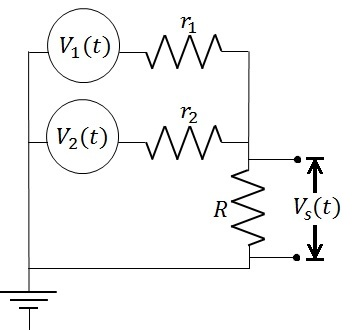
\includegraphics[scale=0.7]{Sumador}
\caption{Circuito sumador con $R>>r_1,r_2$, los valores de $r_1$ y $r_2$ permiten pesar en que proporcion se suma cada coeficiente. En la experiencia se utilizó $r_1 = r_2 \equiv r$ y dos fuentes sinusoidales.}
\label{fig:Sumador}
\end{figure}

Por otro lado, teniendo una señal de entrada con batido $V(t)$, sería válido querer recuperar una de las dos señales $V_1(t)$ o $V_2(t)$ que la componen, eliminando la otra. Aunque podría nuevamente utilizarse el circuito RCL descripto más arriba, un circuito RCL antiresonante (donde la capacitancia $C$ y la inductancia $L$ estan en paralelo) puede resultar más adecuado. Esto es debido a que muchas veces, una señal no sinusoidal $S(t)$ de período $2\tau$ se \textit{modula} utilizando una señal sinusoidal $V_m(t) = A.cos(\omega t)$ (llamada moduladora), generando una nueva señal $S'(t) = S(t)+A.cos(\omega t)$. En este caso, $S(t)$ es una suma de infinitas sinusoides como se explicó más arriba y un RLC resonante solo permitiría que una de estas señales atraviese el filtro.

Un circuito RLC antiresonante, sin embargo, elimina las señales sinusoidales cuya frecuencia sea $\omega_o = \frac{1}{\sqrt{LC}}$. El \textit{ancho de banda} resulta para este caso $\Delta\omega = \frac{1}{(R_L+R)C}$. En resumen,

\begin{equation}
\begin{split}
\omega_o = \frac{1}{\sqrt{LC}}\\
\Delta\omega = \frac{1}{(R_L+R)C}
\end{split}
\label{eq:antiresonante}
\end{equation}

Por lo tanto, si se conoce la frecuencia $\omega$ de la moduladora y se cumple que $|\omega-\frac{pi}{\tau}n|>> \Delta\omega$ $\forall n$, resulta posible recuperar la señal $S(t)$ a la salida del filtro. Para el caso de dos sinusoides, se busca que $|\omega_1-\omega_2|>> \Delta\omega$.


%%%%%%%%%%%%%%%%%%%%%%%%%%%%%%%%%%%%%%%%%%%%%%%%%%%%%%%%%%%%%%%%%%%%%%%%%%%%%%%%%%%%%%%%%%%%%%%%%%%%%%%%%%%%%%%%%%%%%%%%%%%%%%%
% 3. DISPOSITIVO EXPERIMENTAL: armado del modelo, como se midio, consideraciones a la hora de medir.
%%%%%%%%%%%%%%%%%%%%%%%%%%%%%%%%%%%%%%%%%%%%%%%%%%%%%%%%%%%%%%%%%%%%%%%%%%%%%%%%%%%%%%%%%%%%%%%%%%%%%%%%%%%%%%%%%%%%%%%%%%%%%%%

\section{Desarrollo experimental}
Durante esta experiencia se utilizó un generador de funciones de dos canales capaz de generar diferencias de potencial $V(t)$ a frecuencias con un error relativo del $0,01\%$ en un rango entre $1\mu Hz$ y $5MHz$. El voltaje \textit{pico-pico} tiene un error relativo del $1\%$ para el rango de voltaje utilizado ($2V-20V$). Además, se utilizó una resistencia variable por décadas en el intervalo ($1\Omega-11110\Omega$), una capacitancia variable por décadas en el intervalo($1nF-1110\,nF$) y una inductancia variable por décadas en el intervalo ($1mH-1110mH$). Usando un multimetro digital se midieron los valores utilizados en todos estos elementos junto con su precisión que era de la forma $\pm(1\%+2d)$ para la resistencia, $\pm(0.7\%+5d)$ para la capacitancia y ($0.7\% +5d$) para la inductancia; ademas de comprobar la continuidad de los cables utilizados.

Se utilizó además un osciloscopio digital con dos canales de entrada capaces de medir diferencias de potencial entre sus dos terminales en un rango de 2mV a 5V con un error relativo del $3\%$ del valor \textit{pico-pico}. El osciloscopio también contaba con un programa de adquisición de datos el cual permitía importar en una computadora las mediciones en su pantalla para luego ser analizadas. 

A la hora de medir voltaje, fue necesario asegurarse que el cable a tierra del osciloscopio estuviera conectado al cable a tierra el generador de funciones. Cuando se utilizaron ambos canales, se hicieron coincidir las 3 tierras.

\subsection{Análisis de espectro}

Como ya se explicó, para realizar el análisis del espectro de una señal es necesario separar la frecuencia $\omega_n = \frac{n \pi}{\tau}$ y filtrar el resto. Para ello se utilizó un circuito RLC resonante como el que muestra la \textbf{Figura \ref{fig:RLC-espectro}}.

\begin{figure}[h]
\centering
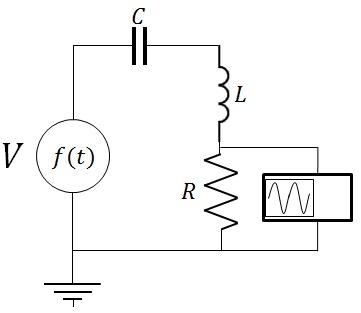
\includegraphics[scale=.7]{RLC-espectro}
\caption{Circuito RLC utilizado para obtener el espectro de frecuencia de Fourier}
\label{fig:RLC-espectro}
\end{figure}

El análisis se realizó para señales $f(t)$  de forma cuadrada y parabólica, las cuales tenían una amplitud$(3.90 \pm 0.02)V$ y $(10.0 \pm 0.2)V$ respectivamente. El objetivo fue poder calcular la trasmisión y obtener los coeficientes dados por \eqref{eq:coef_cuad} y \eqref{eq:coef_parab} en cada caso.

Para ello, al tener en cuenta la importancia del ancho de banda del circuito a la hora de filtrar señales, se usó una resistencia $R=(750 \pm 7)\Omega$ y una inductancia $L=(1003 \pm 5)mH$ la cual aportaba una resistencia $R_L = (243 \pm 2)\Omega$; por lo que de \eqref{eq:resonante} se obtiene $ \Delta f = \frac{\Delta \omega}{2\pi} = (158 \pm 3)Hz$ y una transmisión máxima $T_{max}=(0.75 \pm 0.01)$.

Ademas, es claro que las frecuencias que se desean filtrar son múltiplos de la frecuencia $f_s = \frac{1}{2\tau}$ por lo que no dependen de la forma de la señal. Debido a esto, se impusieron a las dos señales una frecuencia $f_s = (500 \pm 0.05) Hz$ para garantizar la relación $(994\pm 14)Hz=\Delta\omega << \frac{\pi}{\tau} = (3150.0 \pm 0.3)Hz$.

De esta manera, el parámetro $\omega_0$ podía variar únicamente variando la capacitancia $C$, teniendo la frecuencia de resonancia $f_0= \frac{\omega_0}{2\pi}$.

Sabiendo esto, se determinaron los valores de $C$ para que $\omega_0$ coincidiese con los armónicos de $f_s$, como muestra la \textbf{Tabla 1}.

\begin{center}

\begin{tabular}{||c|c|c||}
\hline 
\textbf{Armónico Buscado} & \textbf{Capacitancia $C$ Utilizada (nF)} & \textbf{Frecuencia de resonancia $f_o$ (Hz)} \\ \hline 
 1 & $101 \pm 4$ & $500 \pm 11$ \\ \hline 
 2 & $25,0 \pm 1,3$ & $1005 \pm 29$ \\ \hline 
 3 & $10,7 \pm 0,7$ & $1536 \pm 54$ \\ \hline 
 4 & $6,00 \pm 0,3$ & $2046 \pm 56$ \\ \hline 
 5 & $4,02 \pm 0,19$ & $2506 \pm 65$ \\ \hline 
 6 & $2,98 \pm 0,14$ & $2911 \pm 76$ \\ \hline 
 7 & $1,99 \pm 0,14$ & $3562 \pm 107$ \\ \hline
\end{tabular}
\\[0.3cm] 
\textit{Tabla 1: Capacitancias utilizadas para que $\omega_0$ sea idéntica a los armónicos de $f_s = (500 \pm 0.05) Hz$}

\end{center}

 Y así, para cada uno de ellos, se midió la caída de potencial sobre la resistencia utilizando el osciloscopio. 

Para garantizar que la frecuencia fuera la de resonancia, se hizo un barrido de mediciones en el intervalo de frecuencias $[440,560] Hz$, con el fin de encontrar un máximo de transmisión, para cada $f_0$.


\subsection{Caracterización del sumador}

Para obtener el fenómeno de batido entre señales se utilizaron los dos canales del generador de funciones para armar un circuito \textit{sumador} como el que mostró la \textbf{Figura \ref{fig:Sumador}}, con valores de resistencias $r=(10.5 \pm 0.4)\Omega$ y $R=(200 \pm 3)\Omega$.

Antes de realizar las mediciones en las que se utilizó el \textit{sumador} fue necesario determinar el rango dinámico del mismo. Para ellos, se programaron ambos generadores con una señal triangular con frecuencia $(500 \pm 0.05) Hz$ y una amplitud $(3.00 \pm 0.03)V$.

El objetivo era ver que la amplitud de salida era proporcional al promedio de las amplitudes de entrada; o en caso de no serlo, determinar el rango de voltaje de entrada en el cual la respuesta era lineal. Para ello, al adquirir los datos de la señal de salida, primero se comprobó que tuviera una forma triangular; y luego se calculó la transmisión observando el intervalo donde esta se puede ajustar por una función lineal. Así mismo se determinó si el sumador modificaba la frecuencia de salida, tomando un promedio entre los máximos consecutivos de la señal triangular de salida; y por otro lado, al comparar los tiempos entre máximos de la señal de entrada y salida se pudo ver si había desfasaje entre ellas. 

\newpage
\subsection{Modulación y filtrado}
Una ves hecho esto, se cambiaron las formas de las señales de entrada por una sinusoidal en ambos canales para obtener una señal de salida modulada.

Para filtrar una de las señales de entrada se utilizó un circuito RLC anti-resonante como el que muestra la \textbf{Figura \ref{fig:filtro}}. 

\begin{figure}[h]
\centering
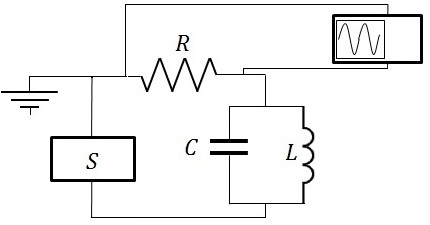
\includegraphics[scale=0.65]{filtro}
\caption{Circuito RLC anti-resonante utilizado para filtrar una de las señales dadas por el sumador \textbf{S}}
\label{fig:filtro}
\end{figure}

Donde el elemento \textbf{S} es el sumador y la diferencia de potencia que entrega es la que sale de sus terminales libres; la resistencia $R=(750 \pm 7)\Omega$, inductancia $L=(10.0 \pm 0.3)mH$ con resistencia $R_L =(5.8 \pm 0.1)\Omega$, y una capacitancia $C=(101,2 \pm 0.8)nF$.

Al quedar fijos estos parámetros, a partir de \eqref{eq:antiresonante} se obtiene una frecuencia de anti-resonancia $f_0 = (5003 \pm 95)Hz$ y un ancho de banda $\Delta f = (2080 \pm 36)Hz$.

Entonces se utilizó una frecuencia $f_1=(10844 \pm 1)Hz$ para un canal, y $f_2=(5003\pm 0.5)Hz$ para el otro, y ambas fuentes con una amplitud $V_0=(3.00 \pm 0.03)V$.



%%%%%%%%%%%%%%%%%%%%%%%%%%%%%%%%%%%%%%%%%%%%%%%%%%%%%%%%%%%%%%%%%%%%%%%%%%%%%%%%%%%%%%%%%%%%%%%%%%%%%%%%%%%%%%%%%%%%%%%%%%%%%%%%
% 4.DISCUSIÓN Y RESULTADOS: todo lo que se obtuvo y explicación. Graficos, tablas.
%%%%%%%%%%%%%%%%%%%%%%%%%%%%%%%%%%%%%%%%%%%%%%%%%%%%%%%%%%%%%%%%%%%%%%%%%%%%%%%%%%%%%%%%%%%%%%%%%%%%%%%%%%%%%%%%%%%%%%%%%%%%%%%%

\section{Resultados}
\label{sec:discusion}

\subsection{Analisis de espectro}
Como se dijo, la señal de entrada era una cuadrada, cuyos coeficientes de Fourier vienen dado por \eqref{eq:coef_cuad}. Sin embargo, para cada valor de $C$, se medían las transmisiones para distintas frecuencias de entrada. Los resultados que se obtuvieron para cada uno de estos barridos se ejemplifican en el gráfico de la \textbf{Figura \ref{fig:armonico1cuad}}, que representa el caso del primer armónico. Aquí puede verse claramente que el máximo se alcanza para $f_s = (500,00 \pm 0,05)Hz$.

\begin{figure}[h]
\centering
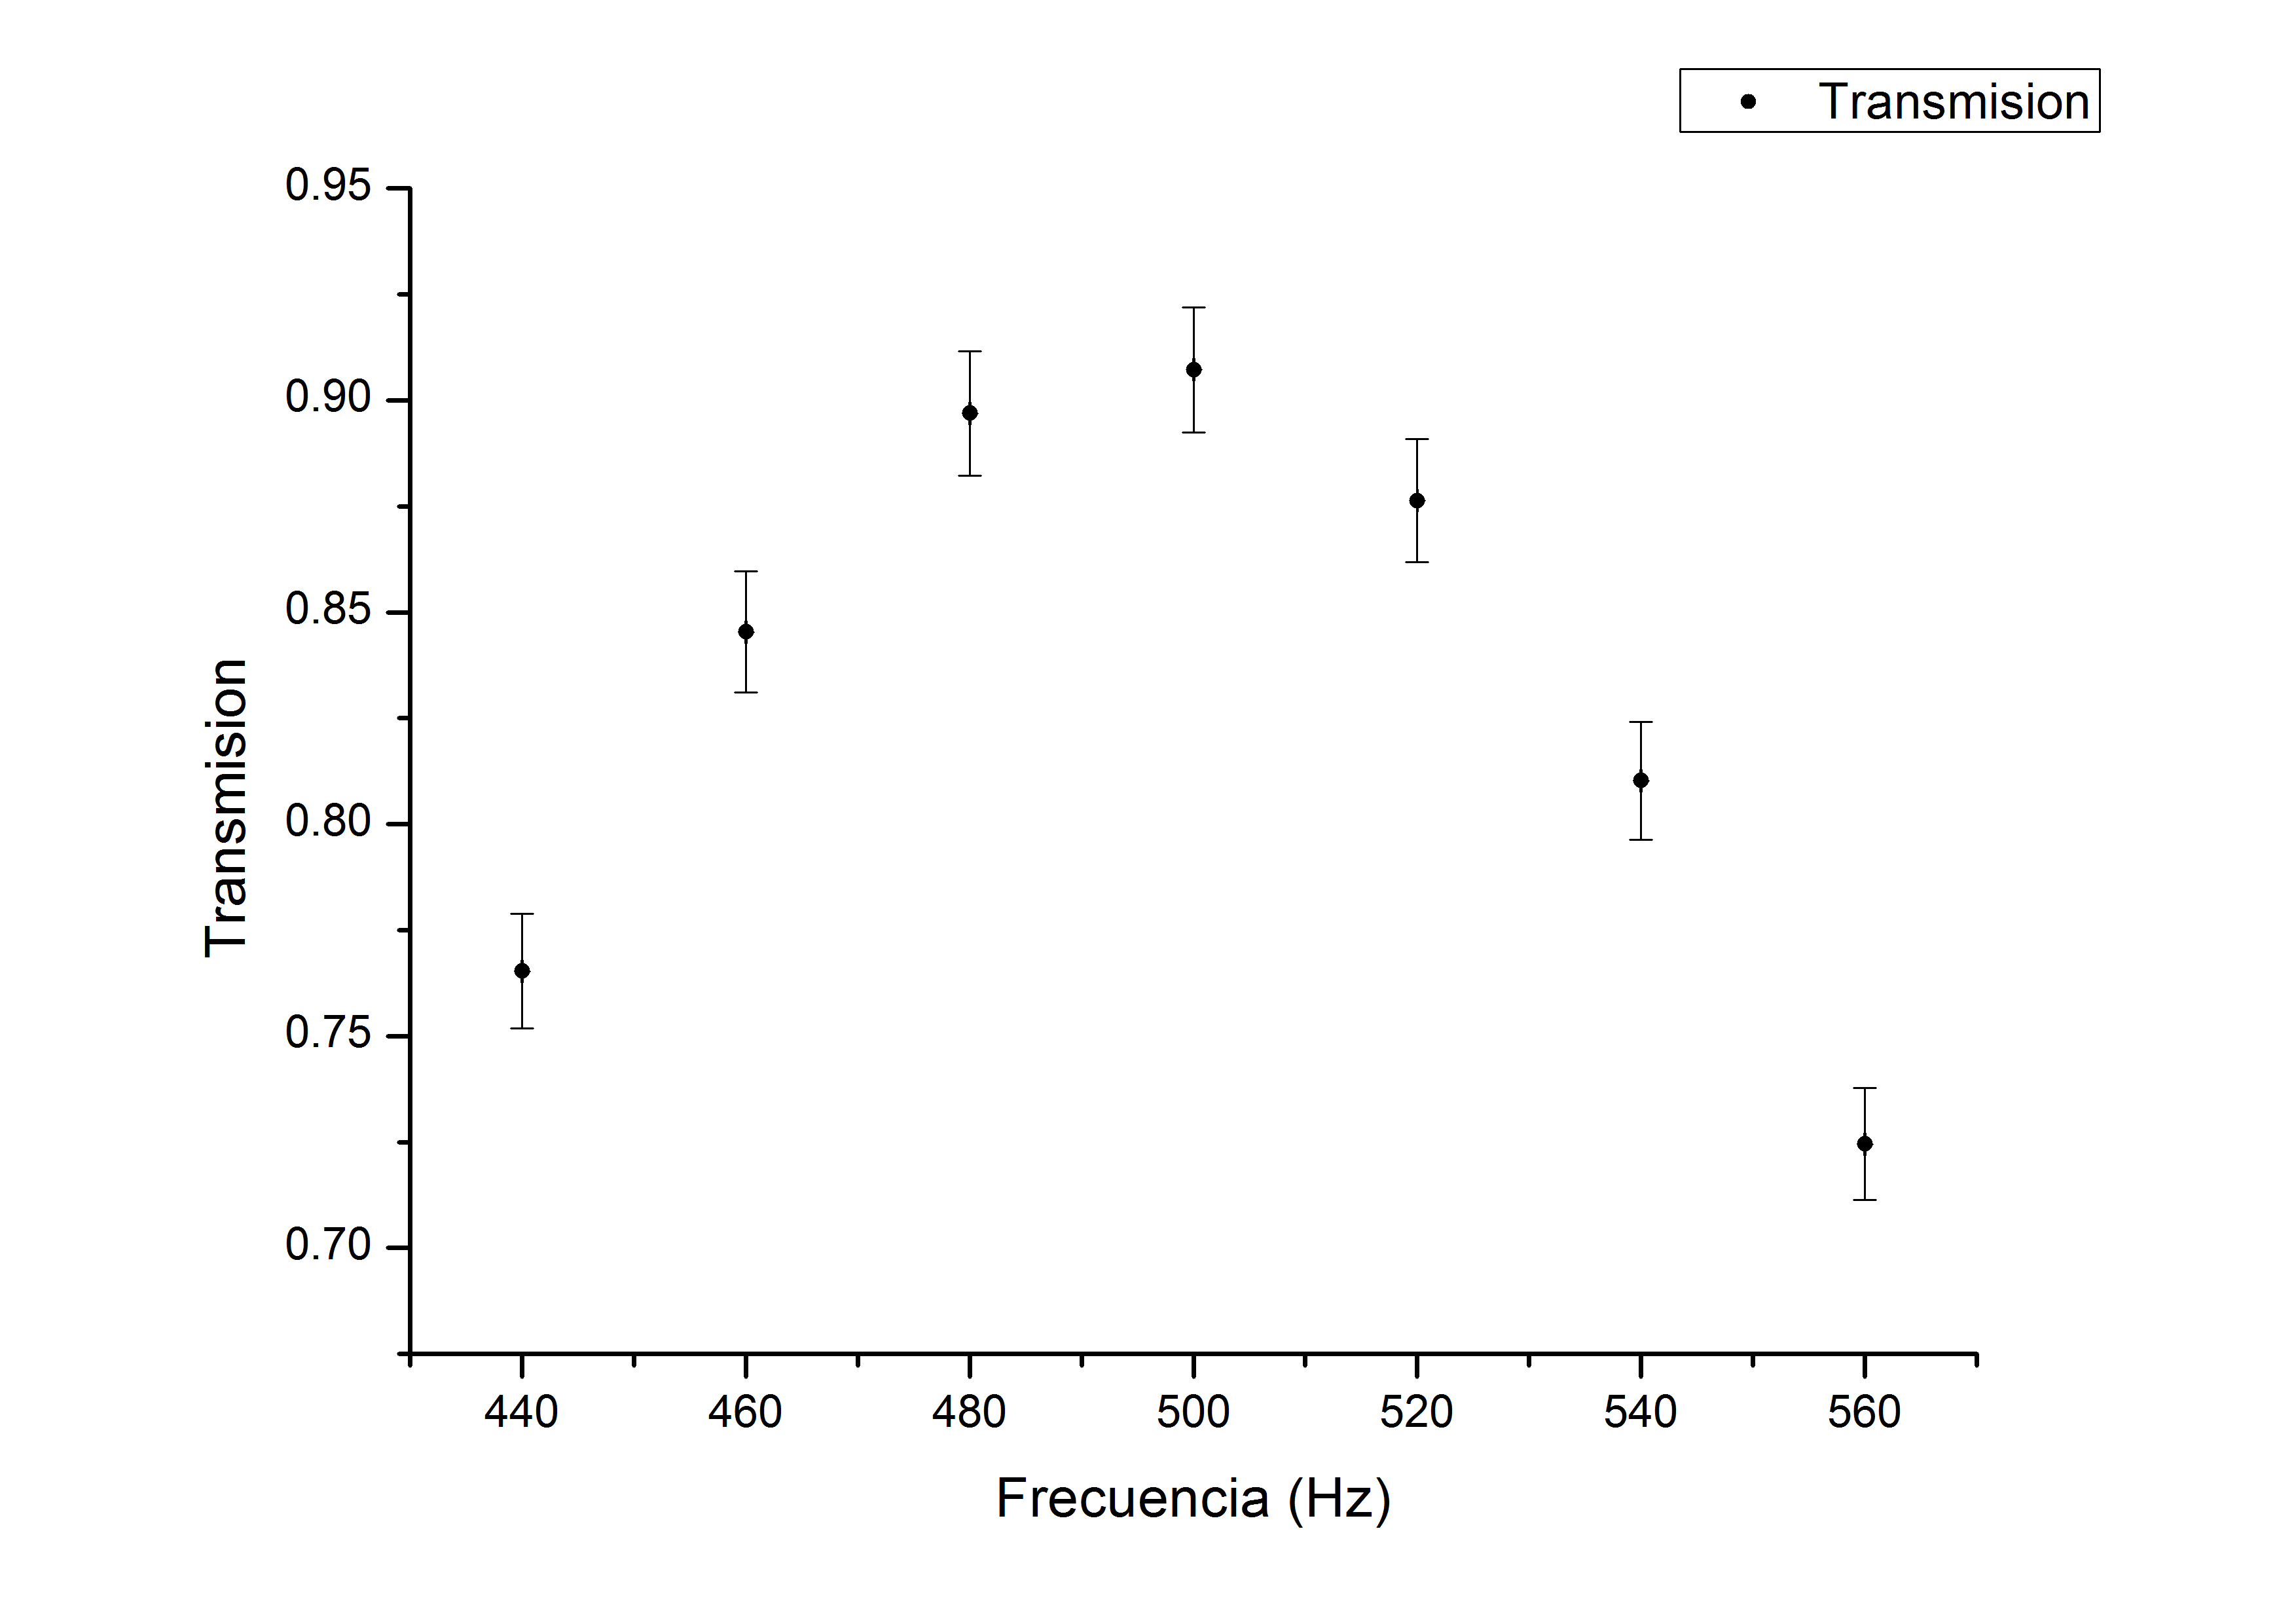
\includegraphics[scale=0.4]{Trans_vs_Frec_Cuad1}
\caption{Grafico de transmisión en función de frecuencia para $f_0 = (500 \pm 11)Hz$ correspondiente al primer armónico}
\label{fig:armonico1cuad}
\end{figure}

Como puede verse en \eqref{eq:coef_cuad}, para los armónicos pares la frecuencia $f_s = (500,00 \pm 0,05)$ debe resultar un máximo mientras que para los impares debe resultar, por lo menos, un mínimo. En todos los casos, el máximo o mínimo (dependiendo del armónico) se halló para $f_s = (500,00 \pm 0,05)$, con excepción del segundo armónico, cuyo mínimo se halló en $f = (490 \pm 10)Hz$ dado que el mismo valor mínimo se halló en $f_s = (480,00 \pm 0,05)Hz$ y en $f_s = (500,00 \pm 0,05)Hz$. El gráfico de la \textbf{Figura \ref{fig:transcuad}} muestra los valores de transmisión para cada armónico impar con su ajuste que arroja un $R-Square = 0,96953$ y un $\chi^2 = 54,38873$ que indican una gran subestimación de errores. Del ajuste se obtiene un $A = (0,91 \pm 0,09)$ que corresponde al valor $T_{max}.\frac{4}{\pi} = (0,962 \pm 0,004)$, cuya diferencia es despreciable frente a los valores manejados, al igual que la ordenada $b =(-0,05 \pm 0,02)$.

\begin{figure}[h]
\centering
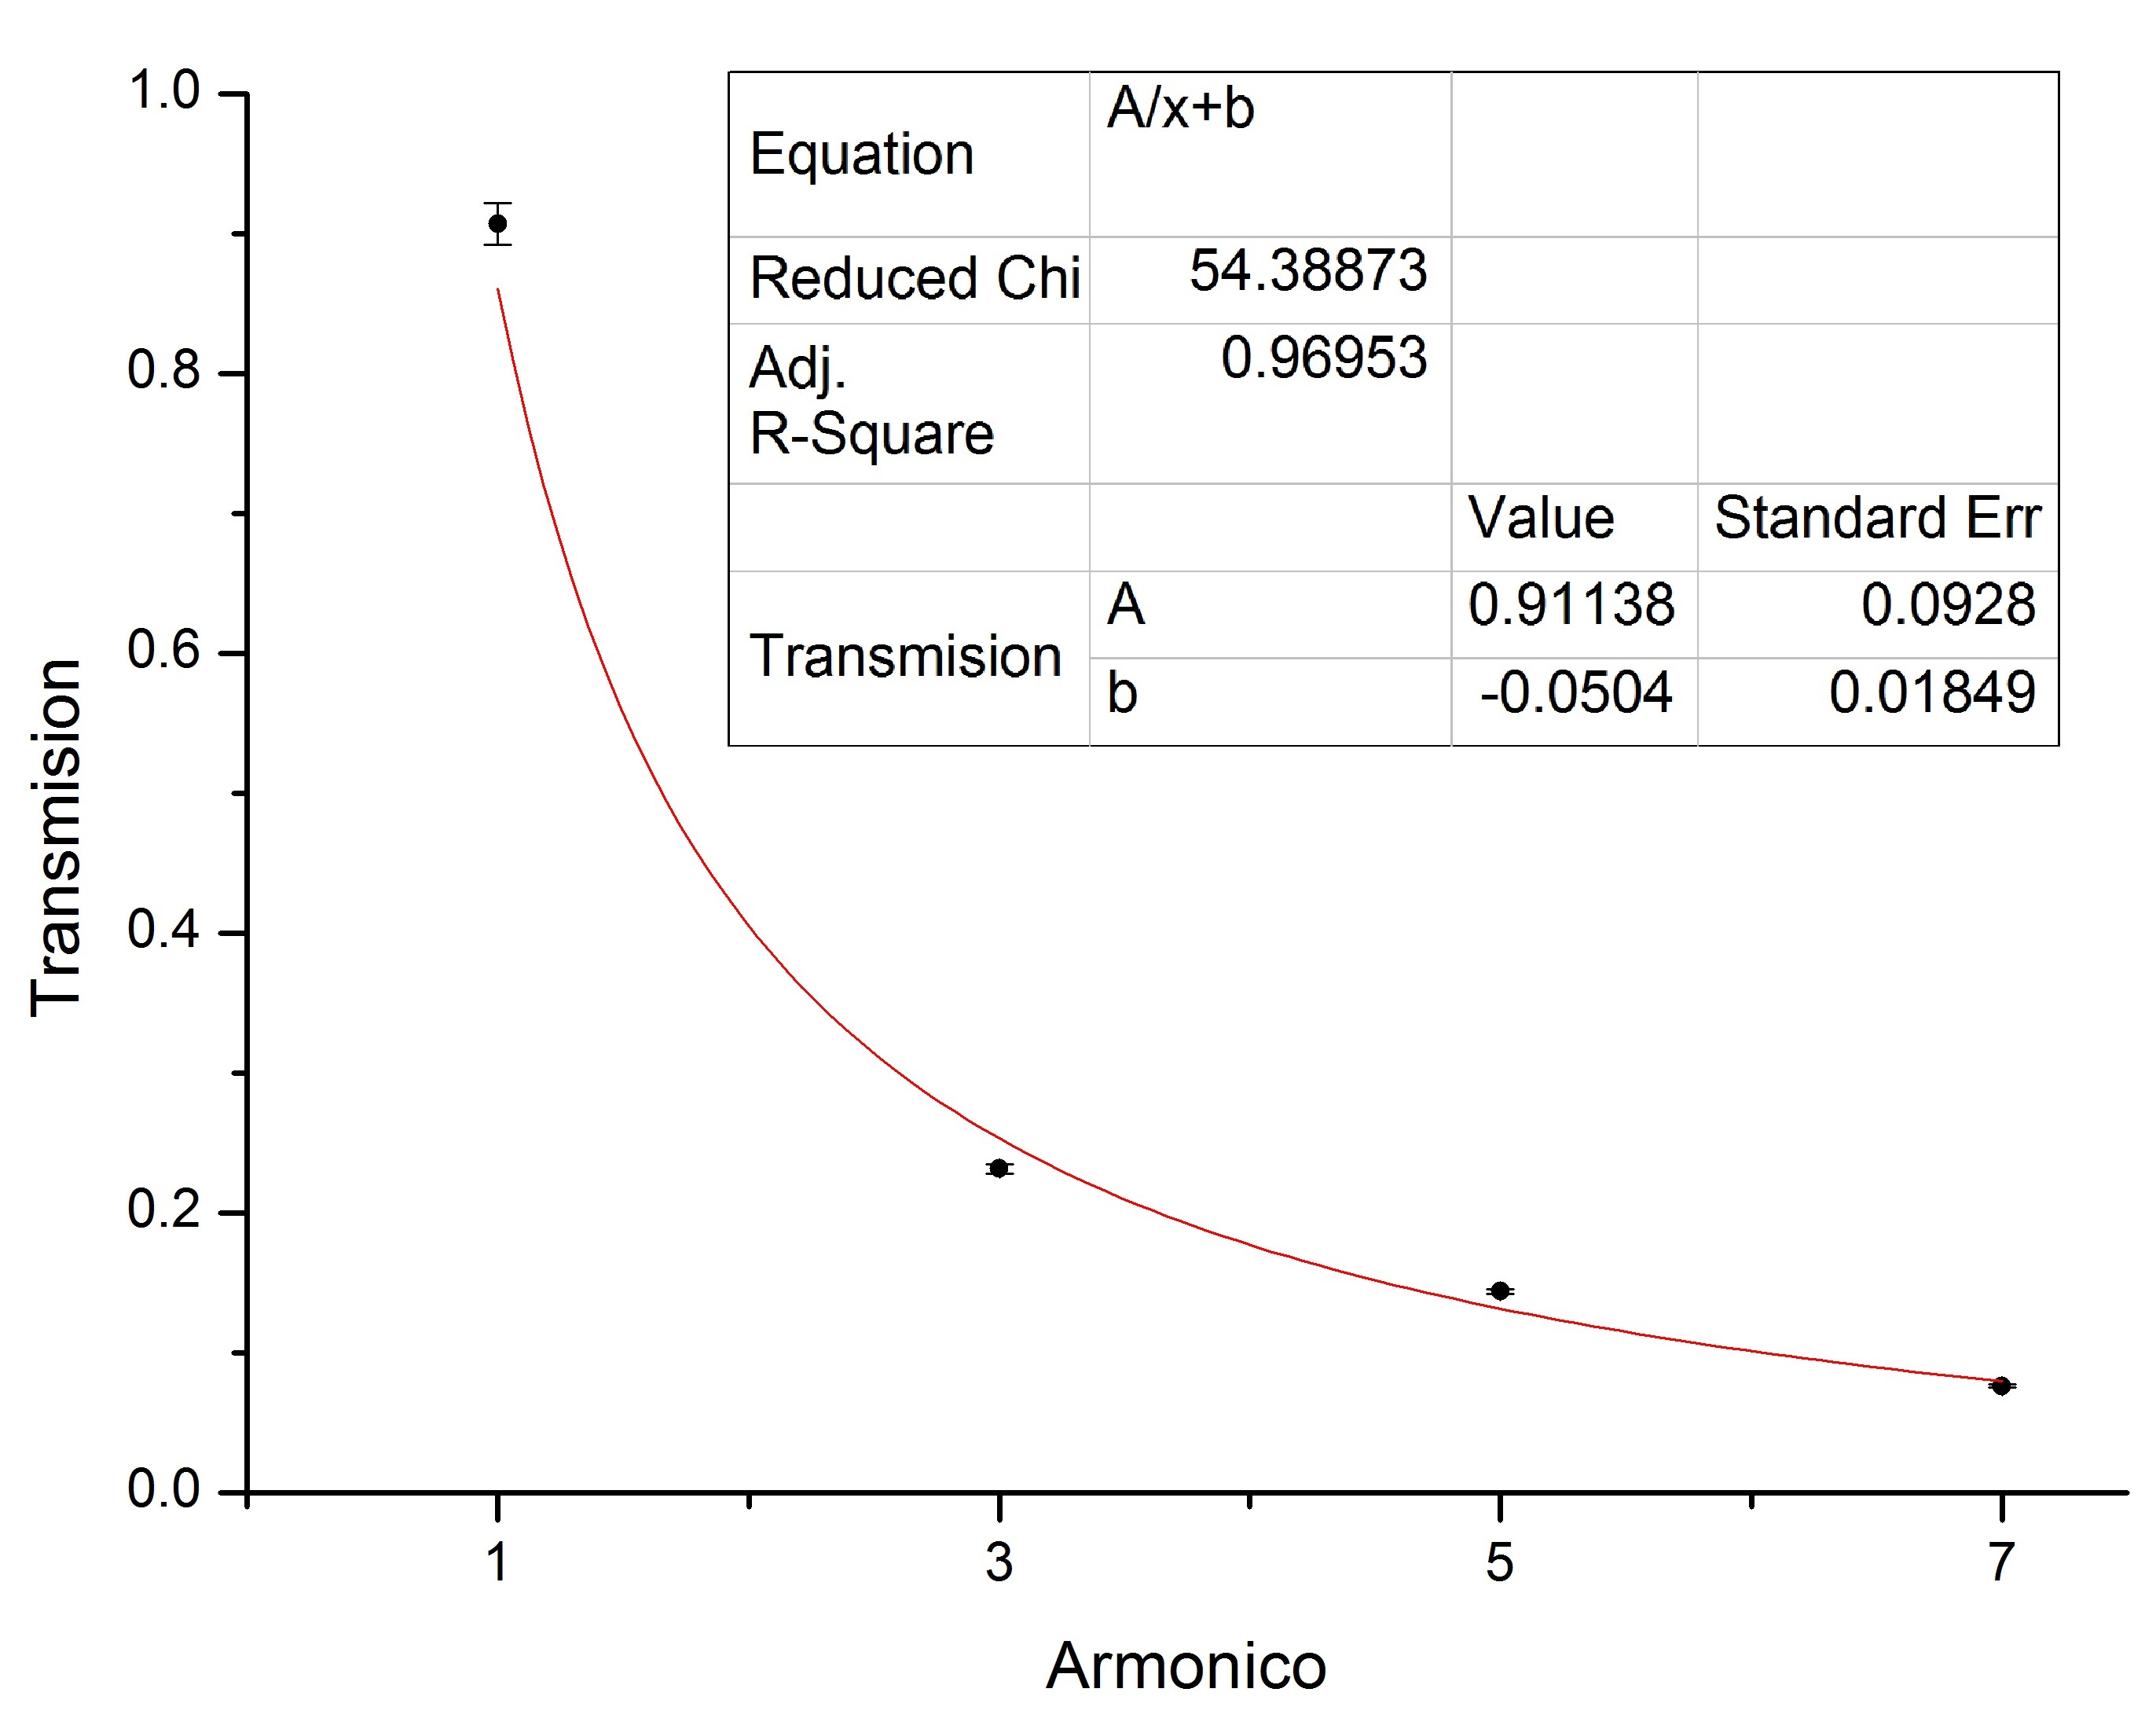
\includegraphics[scale=0.35]{Trans_vs_Arm_Cuad}
\caption{Transmisión en función del armónico analizado, cuyo ajuste arroja los parametros esperados}
\label{fig:transcuad}
\end{figure}

Para el caso de la señal parabólica, la ecuación \eqref{eq:coef_parab} pone a todos los coeficientes en pie de igualdad, por lo que para los distintos valores de $f_o$ se esperaría que $f_s = (500,00 \pm 0,05)Hz$ fuera un máximo de transmisión en el intervalo barrido. Esto se hizo de forma idéntica al análisis de la onda cuadrada, con la diferencia de que no todos los máximos se hallaron en $f_s = (500,00 \pm 0,05)Hz$ como muestra la \textbf{Tabla 2}.

\begin{center}
\begin{tabular}{||c|c||}
\hline 
\textbf{Armónico} & \textbf{Frecuencia de máxima transmisión (Hz)} \\ \hline 
 1 & $500,00 \pm 0,05$ \\ \hline 
 2 & $500,00 \pm 0,05$ \\ \hline 
 3 & $480,00 \pm 0,05$ \\ \hline 
 4 & $480,00 \pm 0,05$ \\ \hline 
 5 & $500,00 \pm 0,05$ \\ \hline 
 6 & $480,00 \pm 0,05$ \\ \hline 
\end{tabular}\\[0.3cm]
\textit{Tabla 2: Frecuencia de máxima transmisión para cada armónico analizado de una señal parabólica. En este caso, no todas las frecuencias son identicas.}
\end{center}

El gráfico de transmisión en función de armónico puede verse en la \textbf{Figura \ref{fig:transparab}}, donde se utilizan los valores de máxima transmisión de cada barrido. Ajustando según \eqref{eq:coef_parab}, arroja un $R-Square = 0,89488$ y un $\chi^2 = 59,20285$, lo cual indica un ajuste medianamente confiable. El parámetro $A = (0,44 \pm 0,07)$ corresponde al parámetro $T_{max}.\frac{4}{\pi^2} = (0,3060 \pm 0,0012)$, donde la diferencia ya no resulta despreciable, aun frente a los errores. Nuevamente, la ordenada $b = (0,011 \pm 0,005)$ resulta despreciable frente a las magnitudes manejadas. Cabe aclarar que el término $(-1)^n$ que aparece en \eqref{eq:coef_parab} se ve absorbido por la fase $\phi_n$ de \eqref{eq:coefs} dado que la prioridad era analizar la amplitud en módulo. 

\begin{figure}[h]
\centering
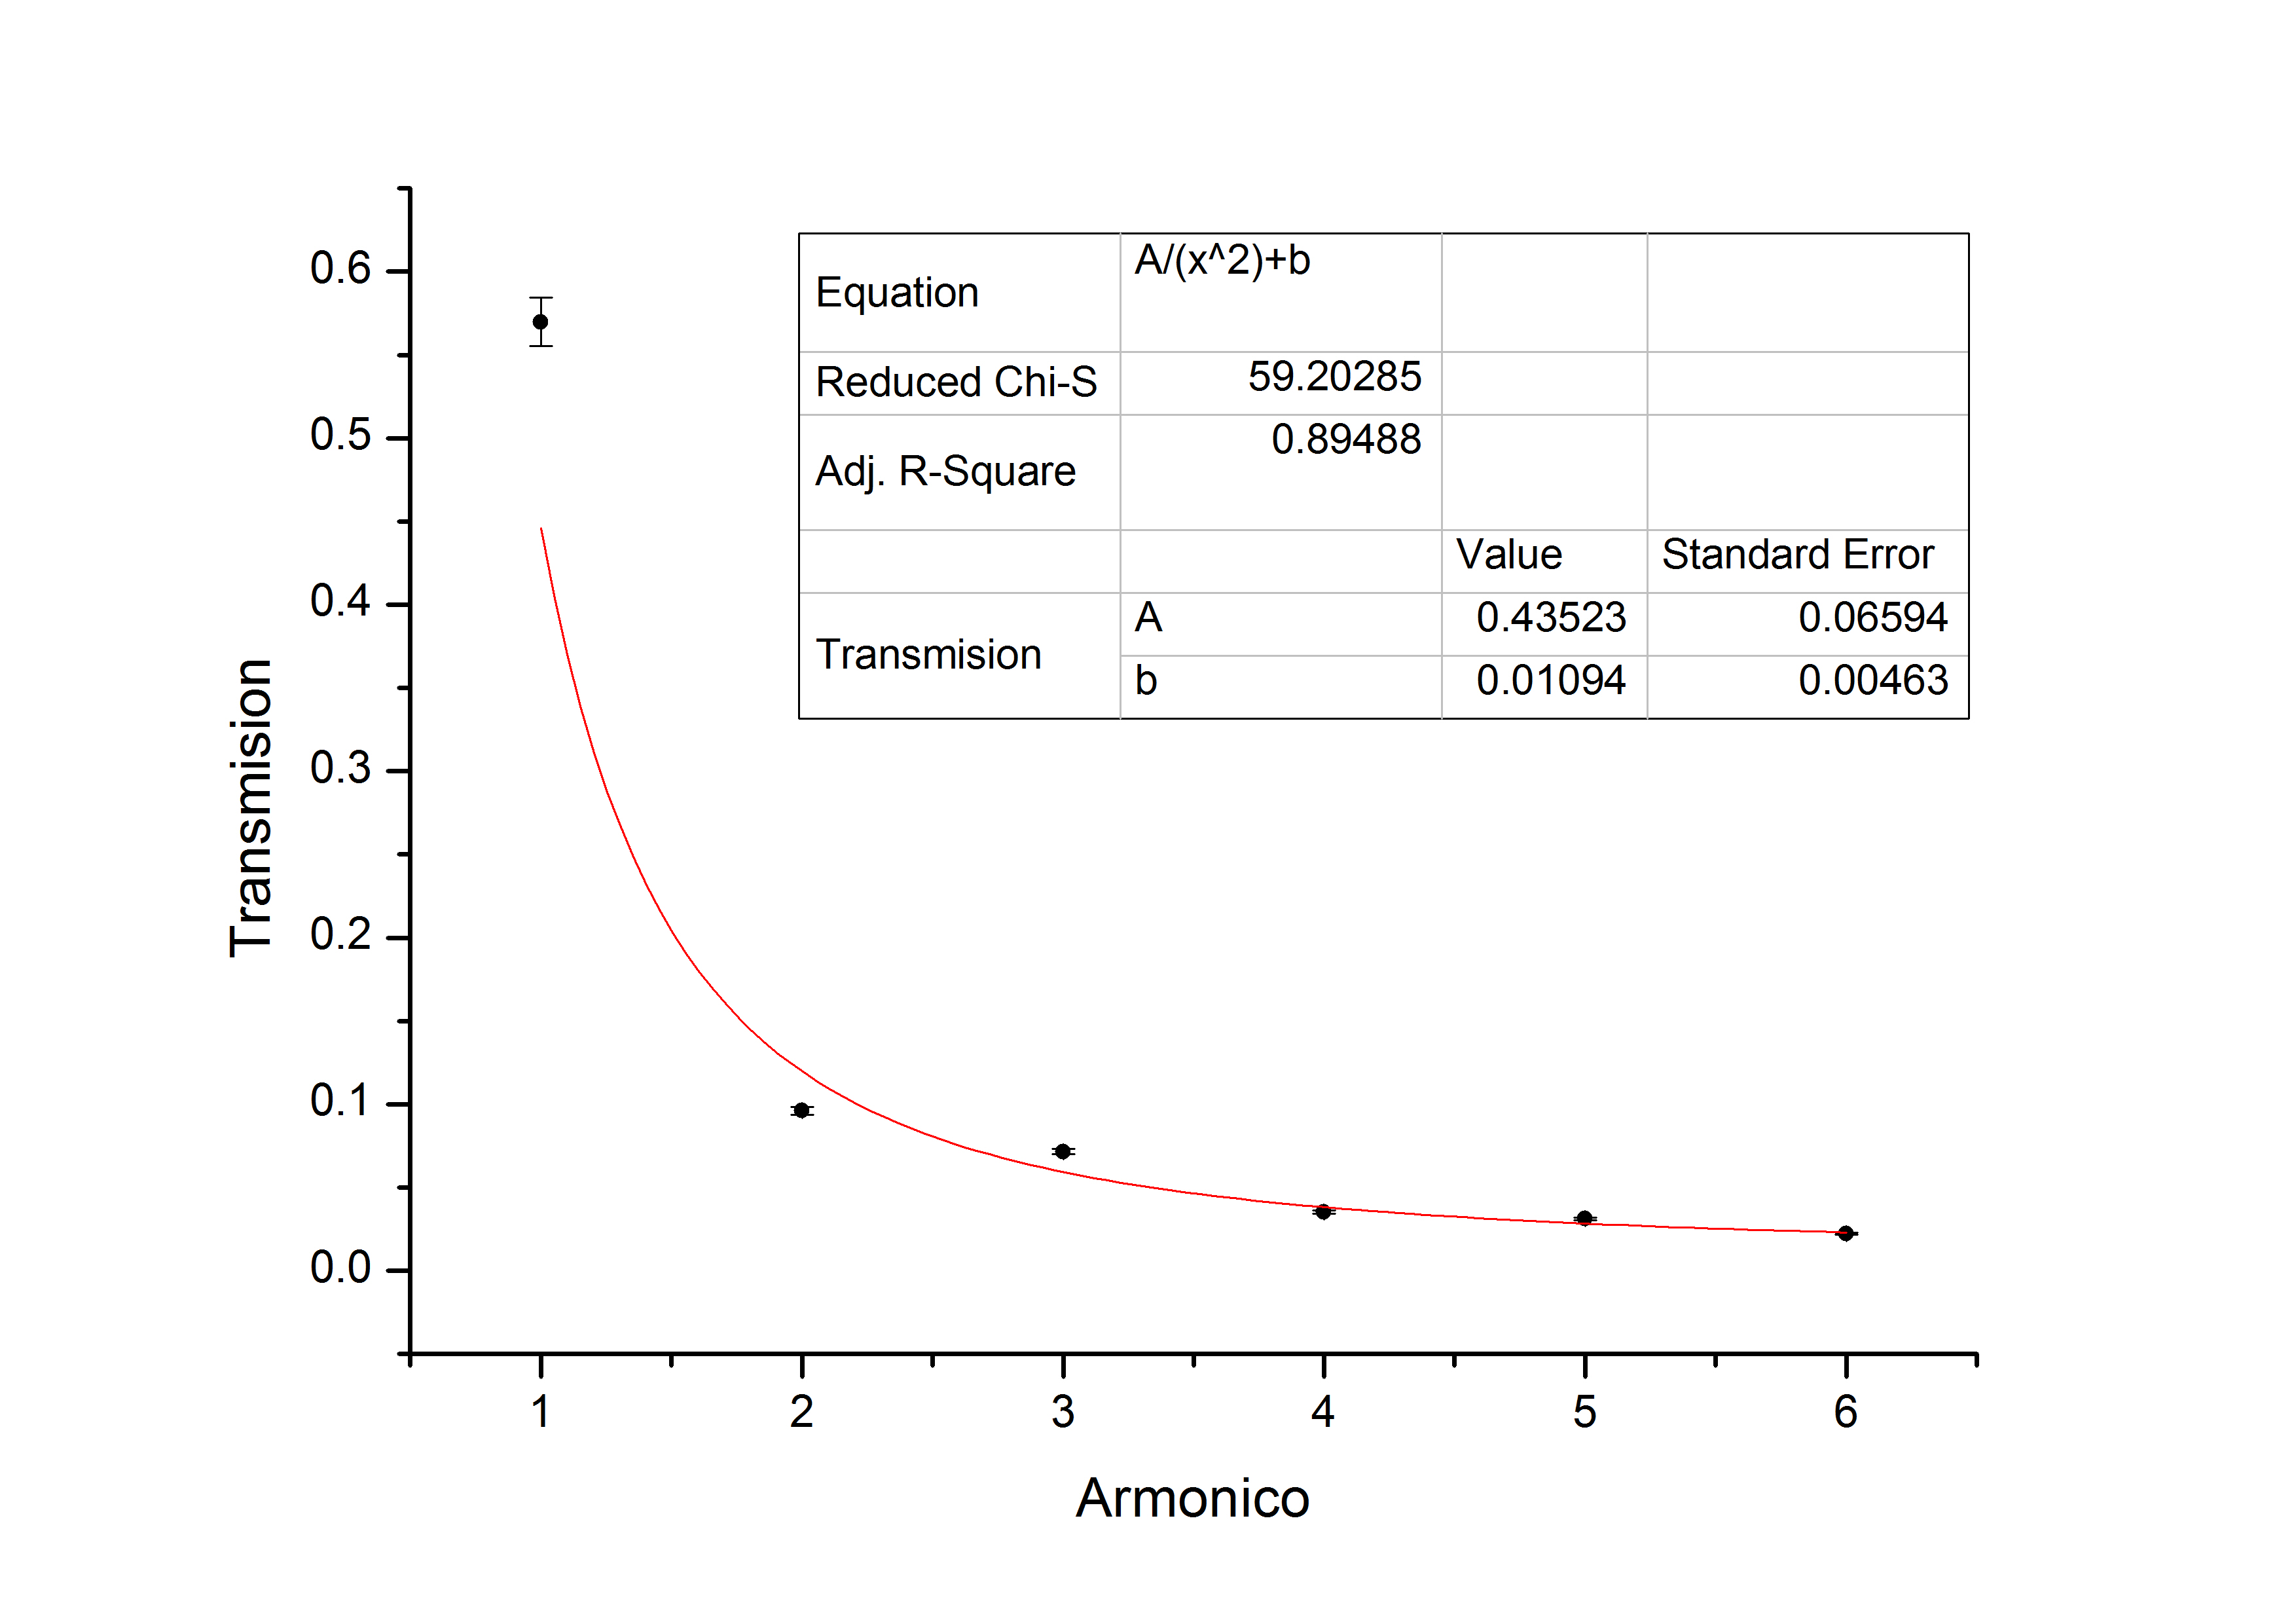
\includegraphics[scale=0.35]{Trans_vs_Arm_Parab}
\caption{Transmisión en función del armónico analizado, donde se utilizaron los valores de transmisión máximos de cada barrido}
\label{fig:transparab}
\end{figure}

\subsection{Caracterización del sumador}

Para caracterizar el sumador, en primer lugar se procedió a chequear que el voltaje de salida sea proporcional a la suma de los voltajes generados por las fuentes. Para esto, se realizó un gráfico que relacionara el voltaje de salida con el voltaje de entrada, como se ve en la \textbf{Figura \ref{fig:S_vs_E}}

\begin{figure}[h]
\centering
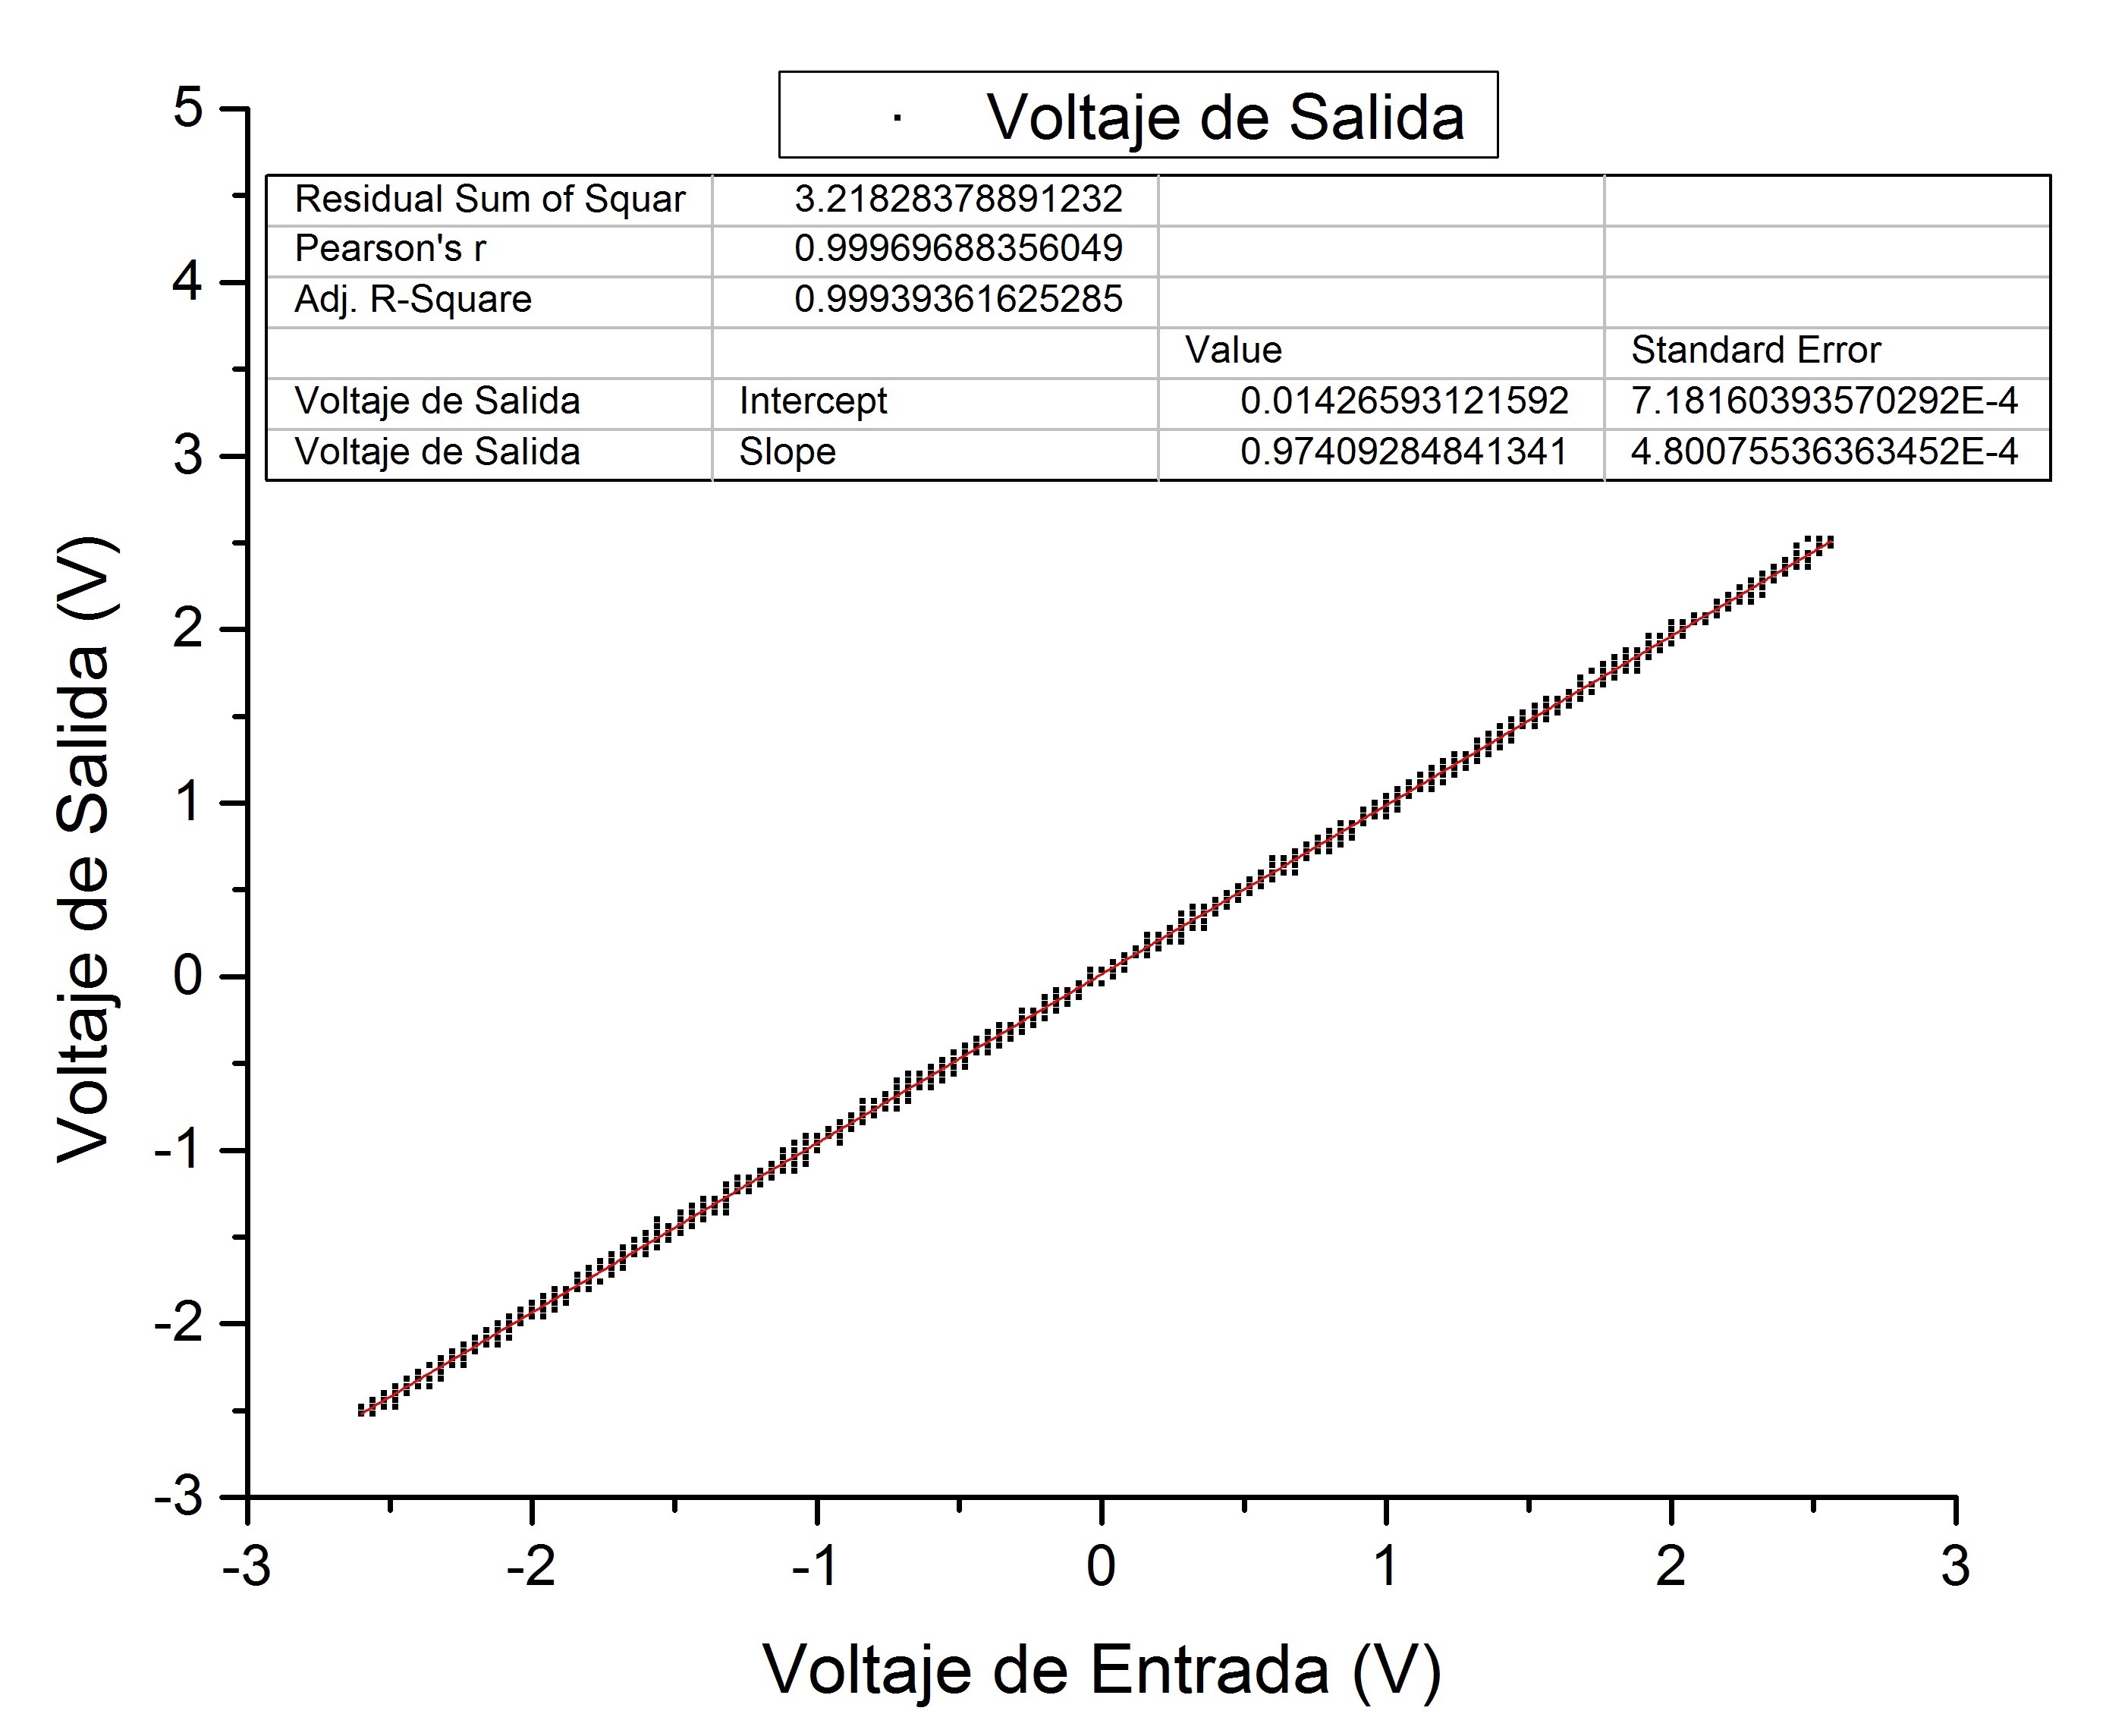
\includegraphics[scale=0.35]{Salida_vs_Entrada}
\caption{Gráfico que muestra la relación entre el voltaje de salida y el de entrada para un circuito con las características ilustradas en la \textbf{Figura \ref{fig:Sumador}}}
\label{fig:S_vs_E}
\end{figure}

Se puede ver que la relación es lineal. Además, el ajuste realizado confirma esa suposición, ya que arroja un $R-Square=0.99939$. Teniendo entonces que la pendiente obtenida del ajuste es el factor de proporción del sumador, que resulto de $(0.9741 \pm 0.0005)$. 

Posteriormente se construyó un gráfico de la señal de salida como se muestra en la \textbf{Figura \ref{fig:Vol_Sal}}, y se relevaron los extremos a fin de poder encontrar la frecuencia con la que estos se repetían.

\begin{figure}[h]
\centering
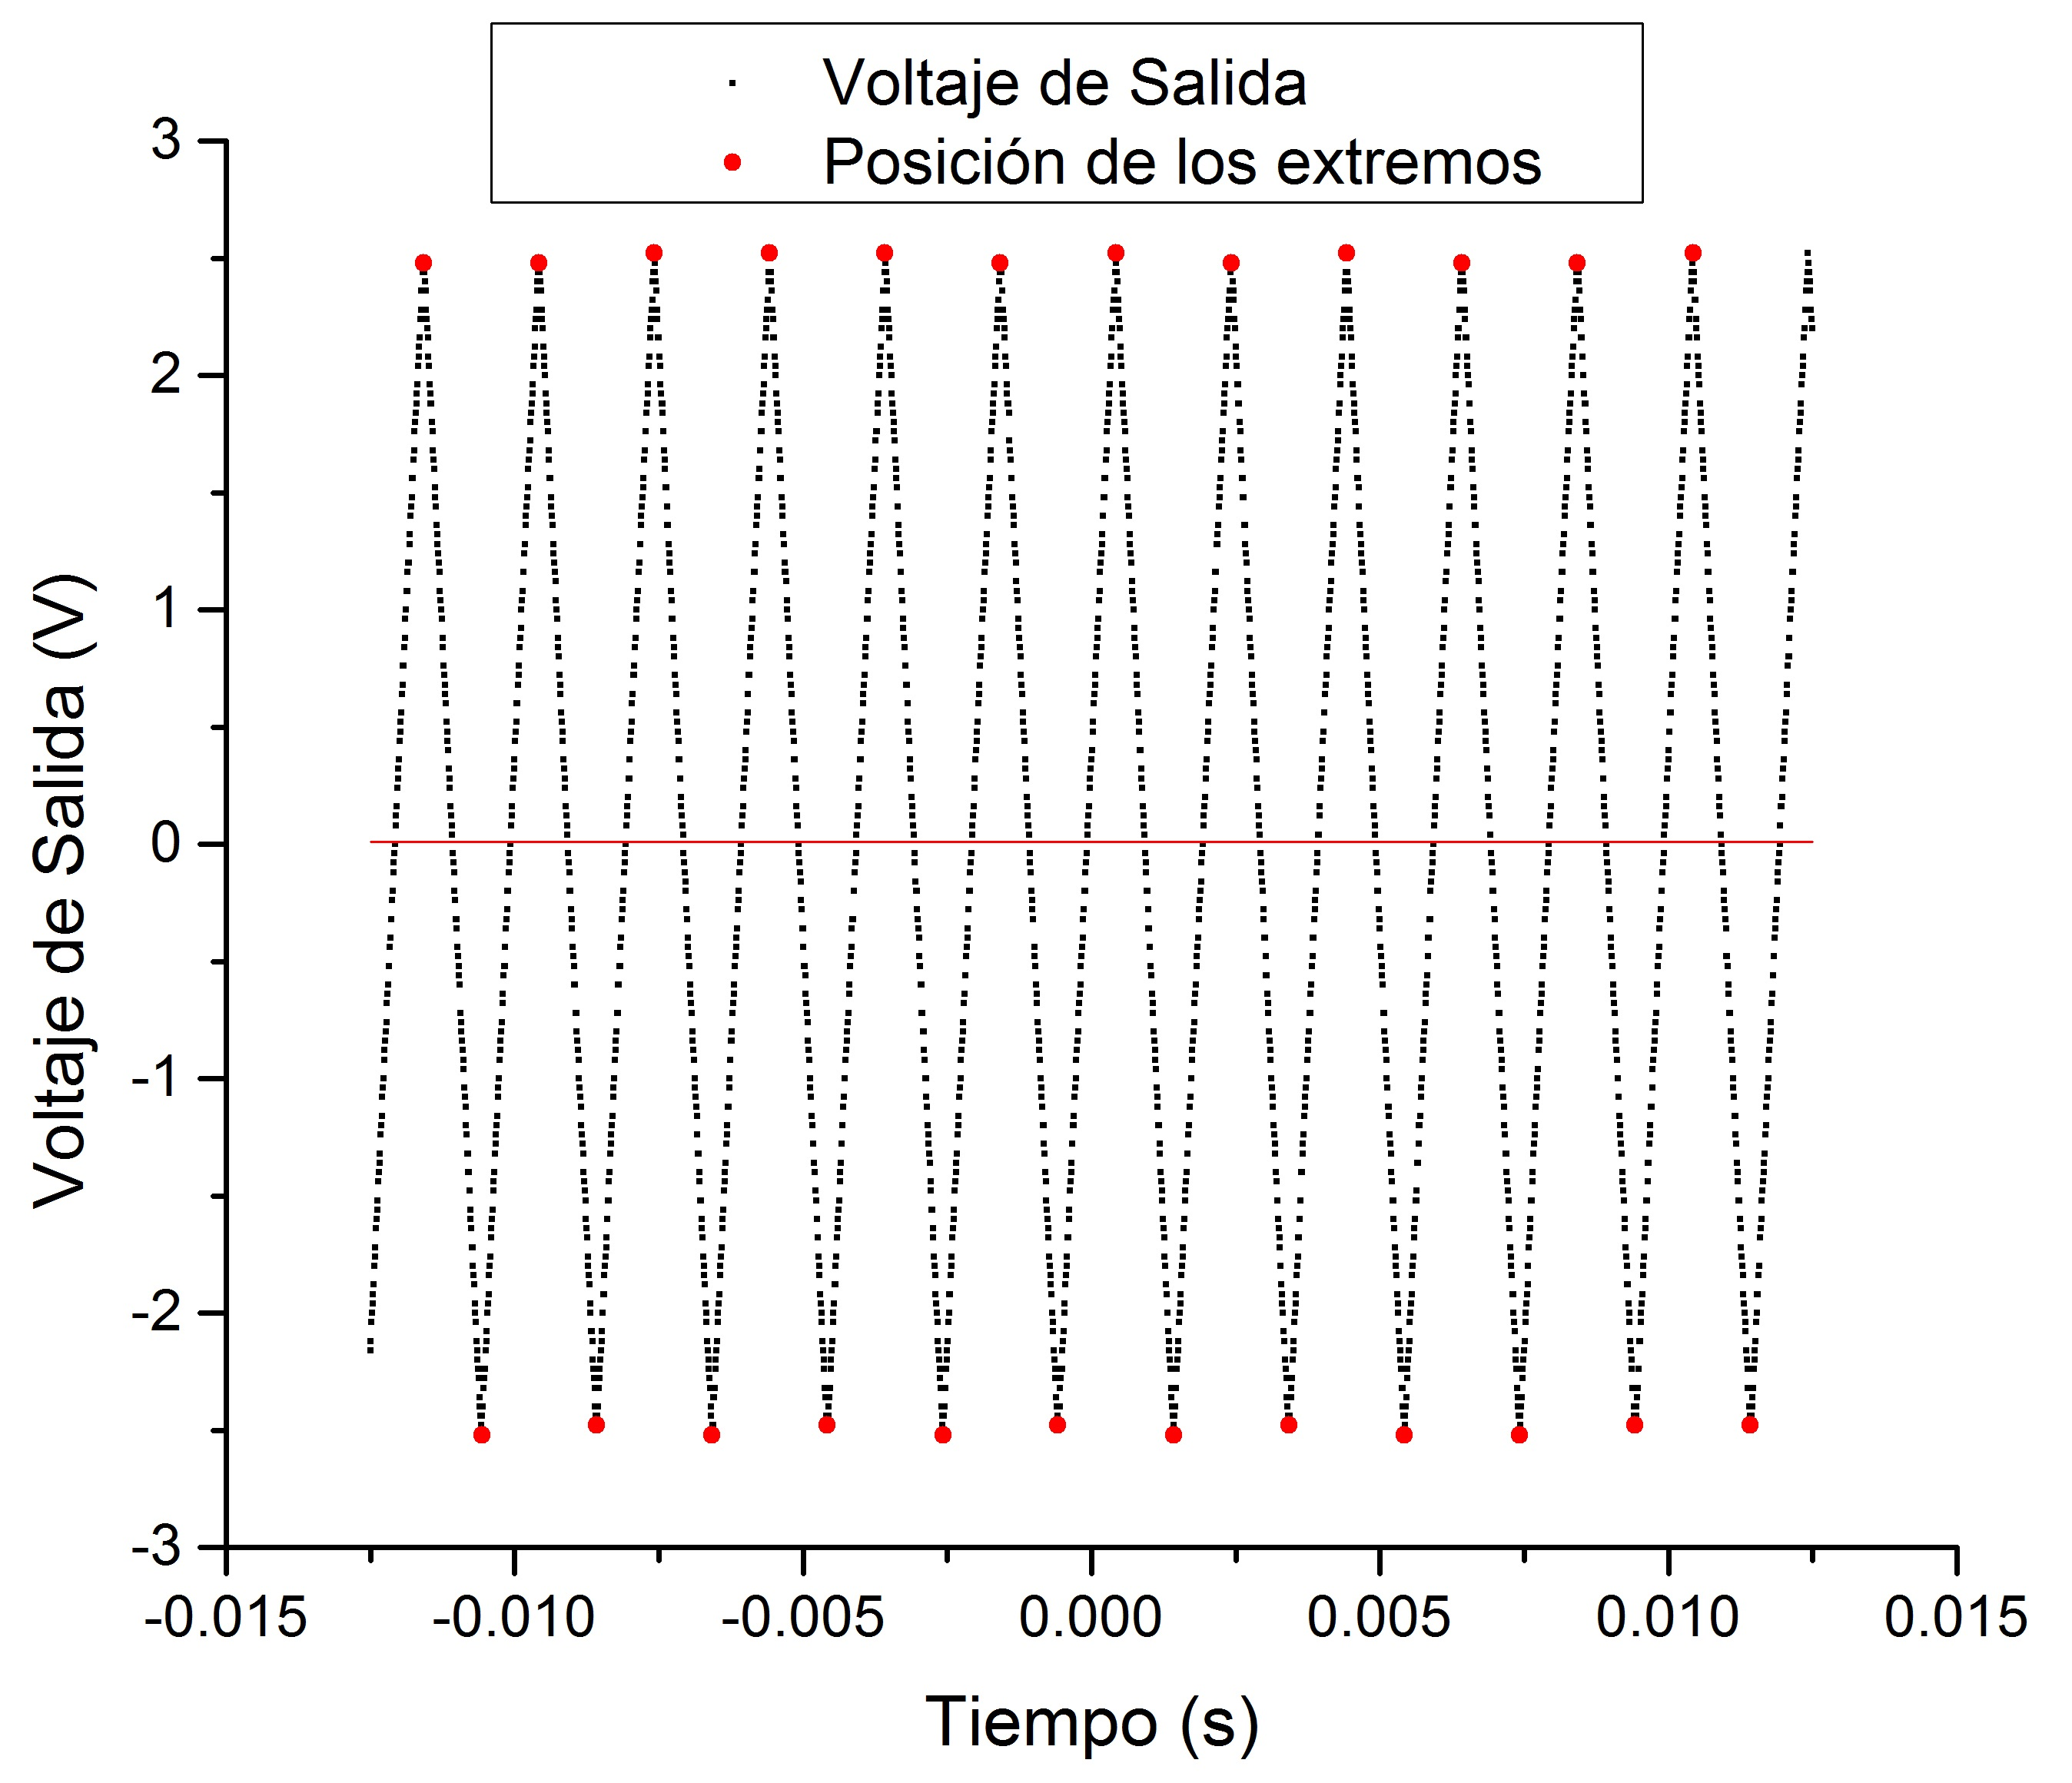
\includegraphics[scale=0.35]{Voltaje_de_Salida}
\caption{Gráfico que muestra el voltaje de salida en funcion del tiempo. Los puntos de mayor tamaño marca la posicion de los extremos.}
\label{fig:Vol_Sal}
\end{figure}

Con los datos obtenidos de los máximos, y luego de los mínimos, se calculó la diferencia entre cada par de valores consecutivos para obtener su periodo, para luego hacer un promedio y obtener la frecuencia $f= (500 \pm 1)hz$ que, como se esperaba, coincide con la utilizada.

Finalmente, se verificó que el sumador no provocara ningún desfasaje en la señal de salida. Para esto realizó un gráfico de la señal de entrada en función del tiempo, que resulto idéntico al del voltaje de salida, y se relevó la posición de los extremos del mismo. Luego se los comparó, con las posiciones encontradas anteriormente, y la diferencia obtenida $D= (2 \pm4)\mu s$ es el desfasaje provocado por el sumador. El cual resultó tres ordenes de magnitud menor que el periodo $\tau = (2 \pm 0.004)ms$ utilizado, por lo cual se lo consideró despreciable.


\subsection{Modulación y filtrado}

Para esta parte de la experiencia se realizaron batidos entre distintas señales. La \textbf{Figura \ref{fig:5_6}} muestra el resultado de enviar dos señales sinusoidales distintas con el \textit{sumador}.

\begin{figure}[H]
\centering
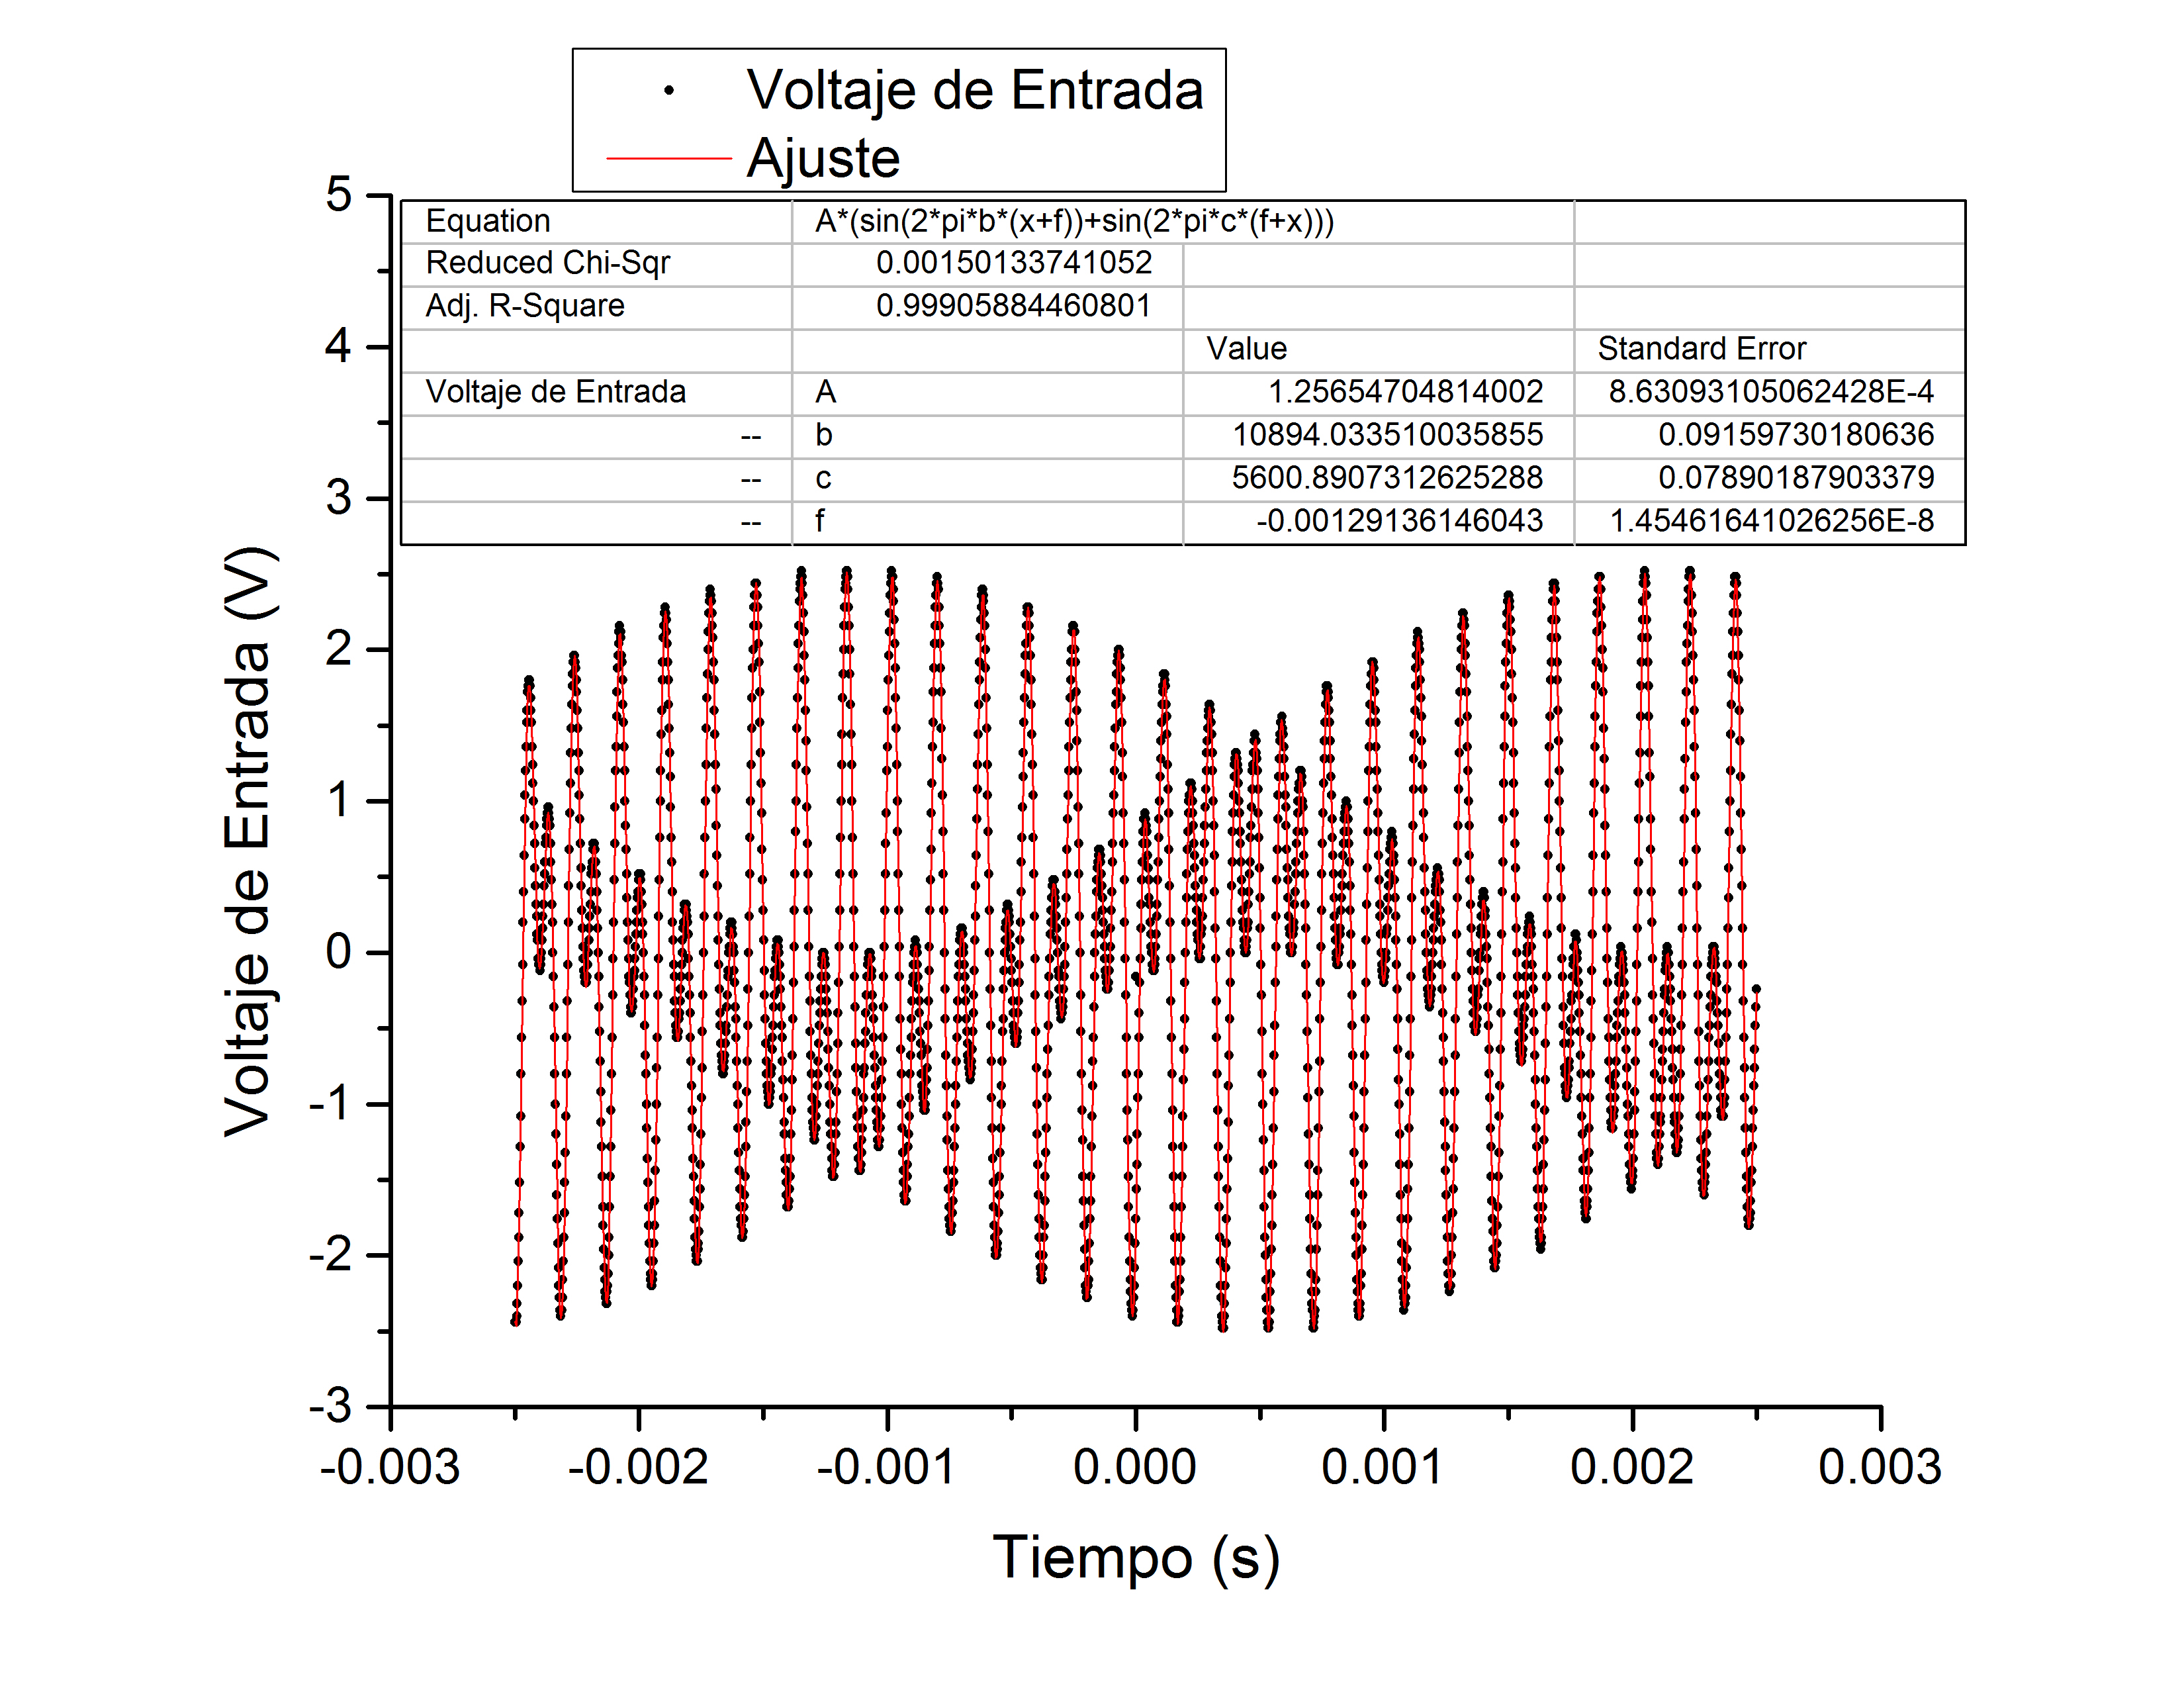
\includegraphics[scale=0.5]{5600hz.jpg}
\caption{Gráfico que muestra el resultado de enviar dos señales sinusoidales distintas con el dispositivo ilustrado en la \textbf{Figura \ref{fig:Sumador}}.}
\label{fig:5_6}
\end{figure}

Sobre el gráfico se realizó un ajuste utilizando una suma de senos para verificar que efectivamente sea lo que se esperaba. Tanto el coeficiente de $R-Square = 0.99906$ muy cercano a uno, como los valores para la frecuencia alta $b = (10894.03 \pm 0.09)hz$ y baja $c = (5600.89 pm 0.08)hz$ que coinciden con las utilizadas, certifican que se obtuvo la señal que se buscaba.

Esta señal se envió a través del circuito ilustrado en la \textbf{Figura \ref{fig:filtro}}, y se midió a la salida lo que se muestra en la \textbf{Figura \ref{fig:5_6_Filt}}. Como se puede ver en la figura antes mencionada, no se puede apreciar alguna diferencia importante entre los dos graficos. Esto era de esperarse ya que la frecuencia de corte del circuito anti-resonante era de $f= (5003 \pm 95)hz$ y no coincide con ninguna de las dos.

\begin{figure}[H]
\centering
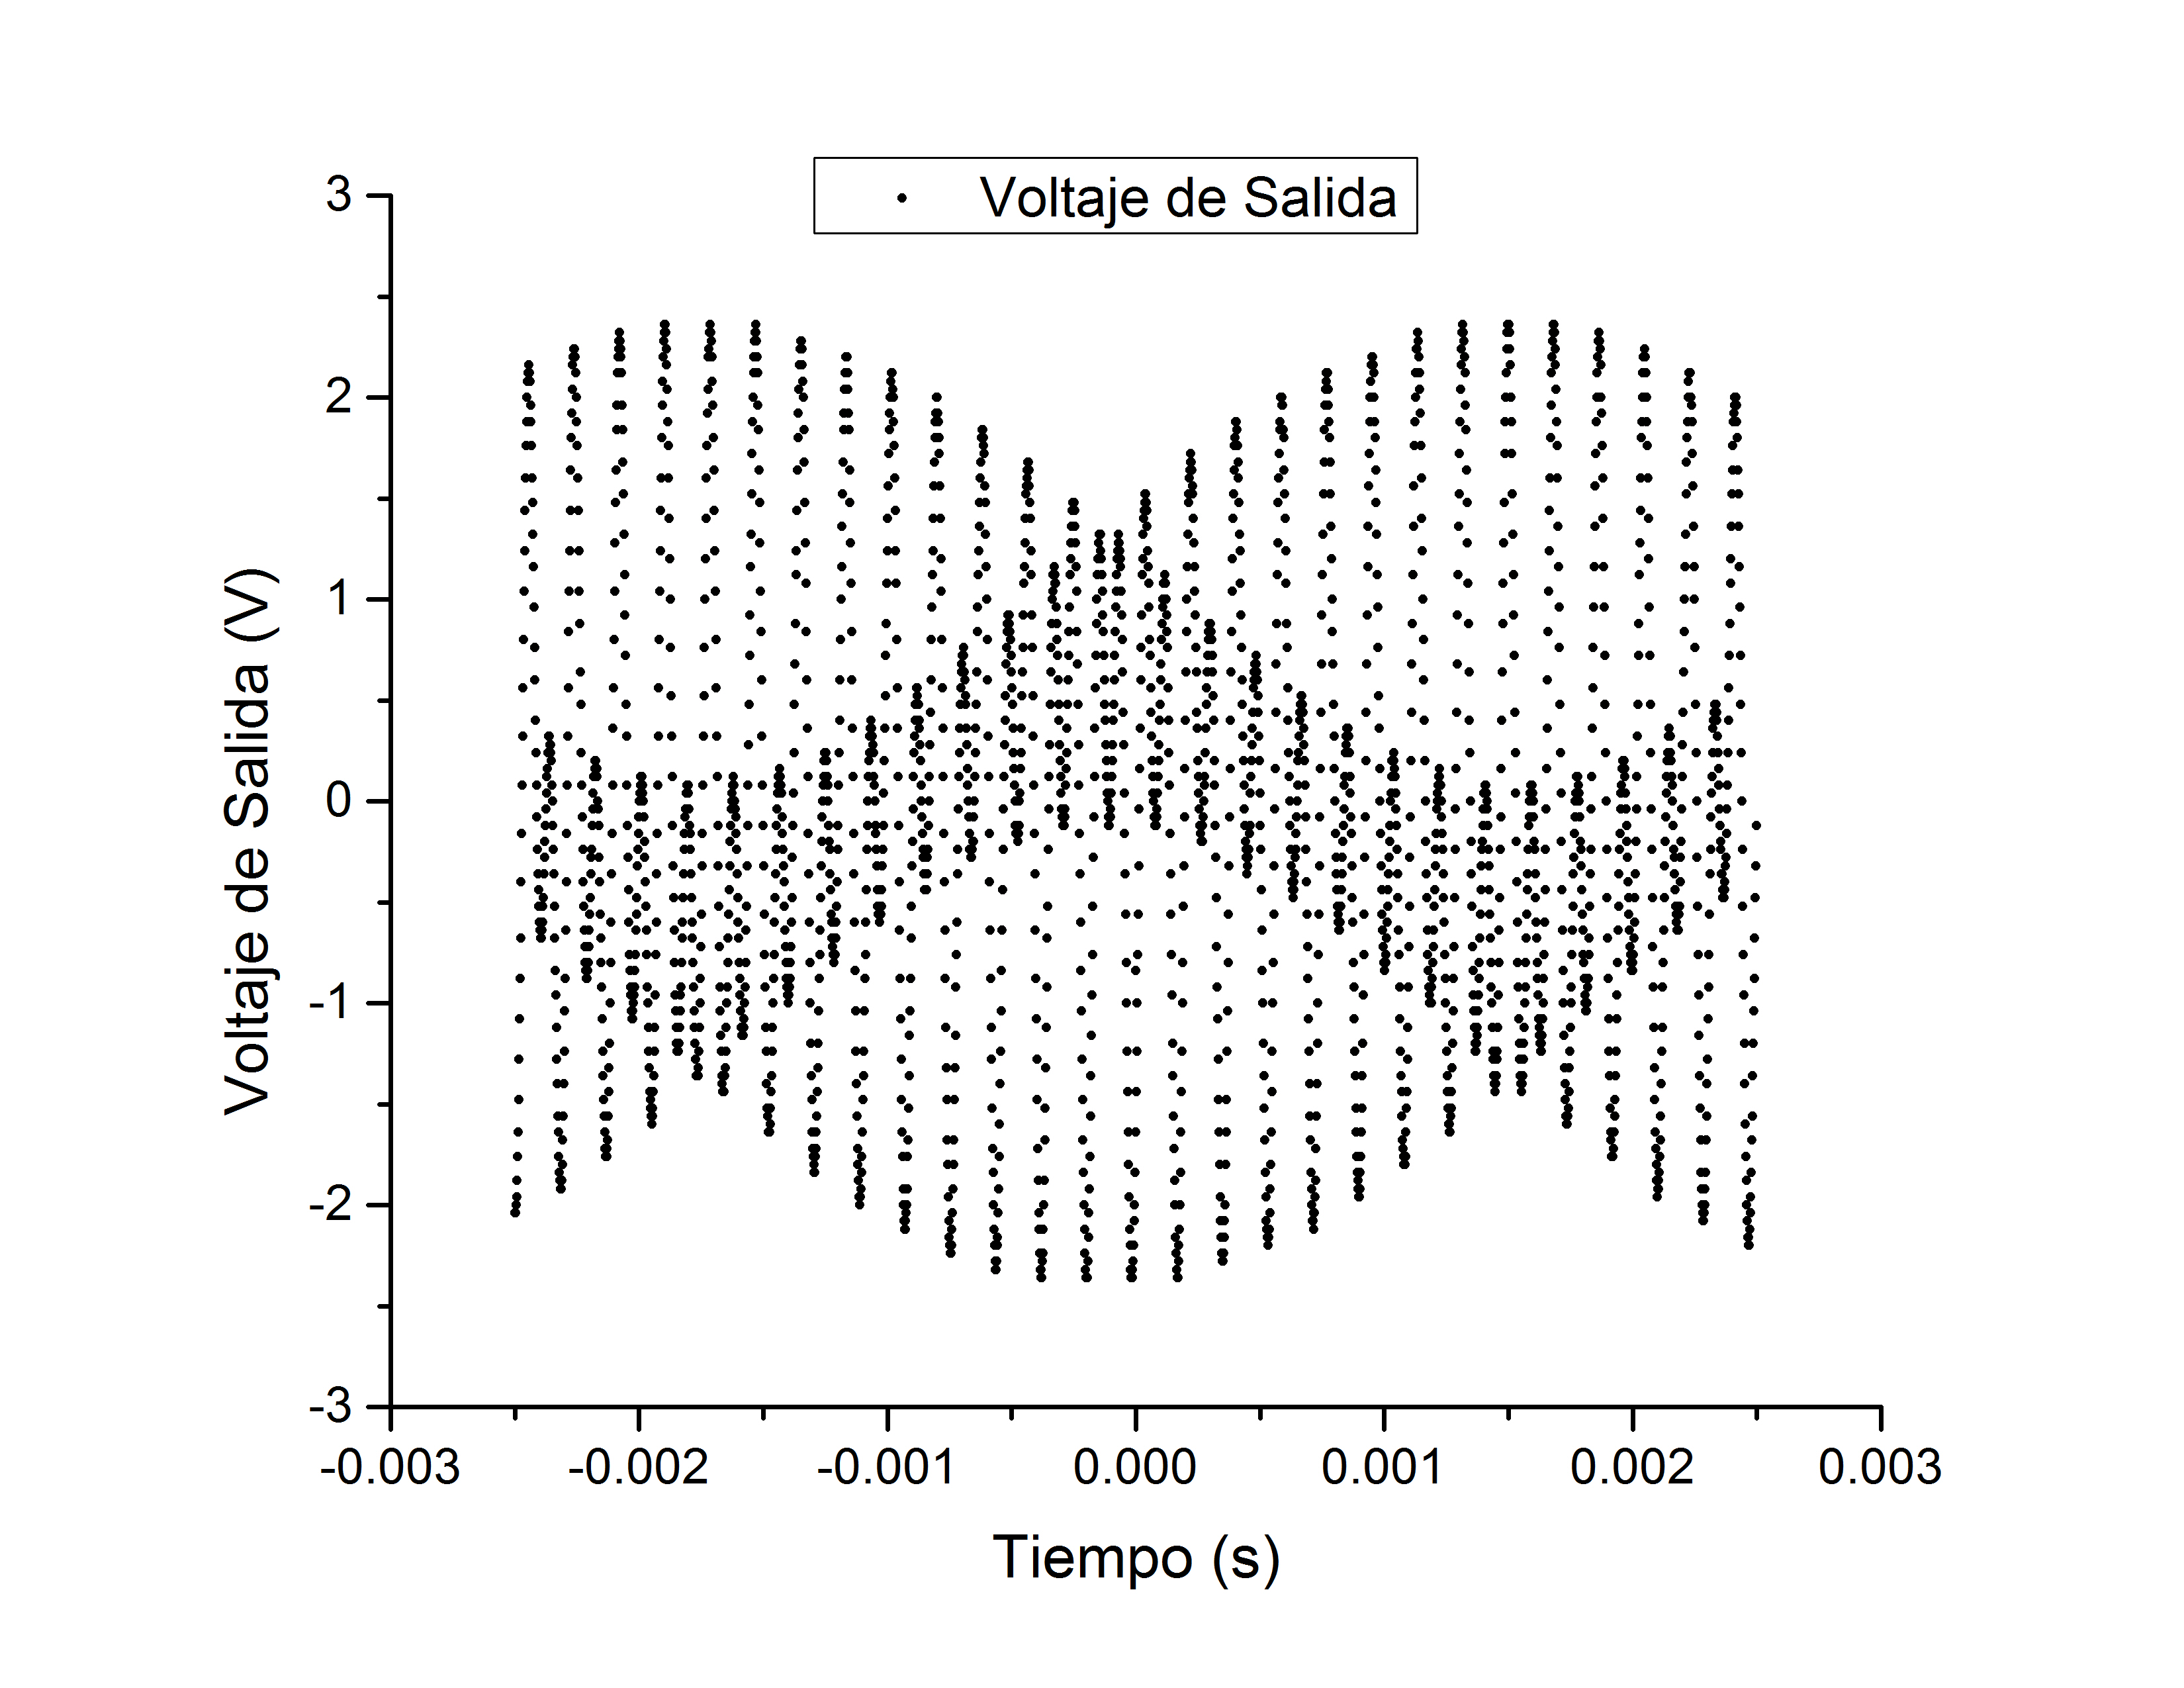
\includegraphics[scale=0.5]{5600hz_Filtrado}
\caption{Gráfico que muestra el resultado de enviar la señal de la \textbf{Figura \ref{fig:5_6}} a travez de un circuito RCL anti-resonante utilizado como filtro.}
\label{fig:5_6_Filt}
\end{figure}

Para una frecuencia baja más cercana a la frecuencia de corte $f= (5005.5 \pm 0.1)hz$ se obtuvieron los graficos de la \textbf{figura \ref{fig:5k}}

\begin{figure}[H]
	\begin{subfigure}{0.5\textwidth}
		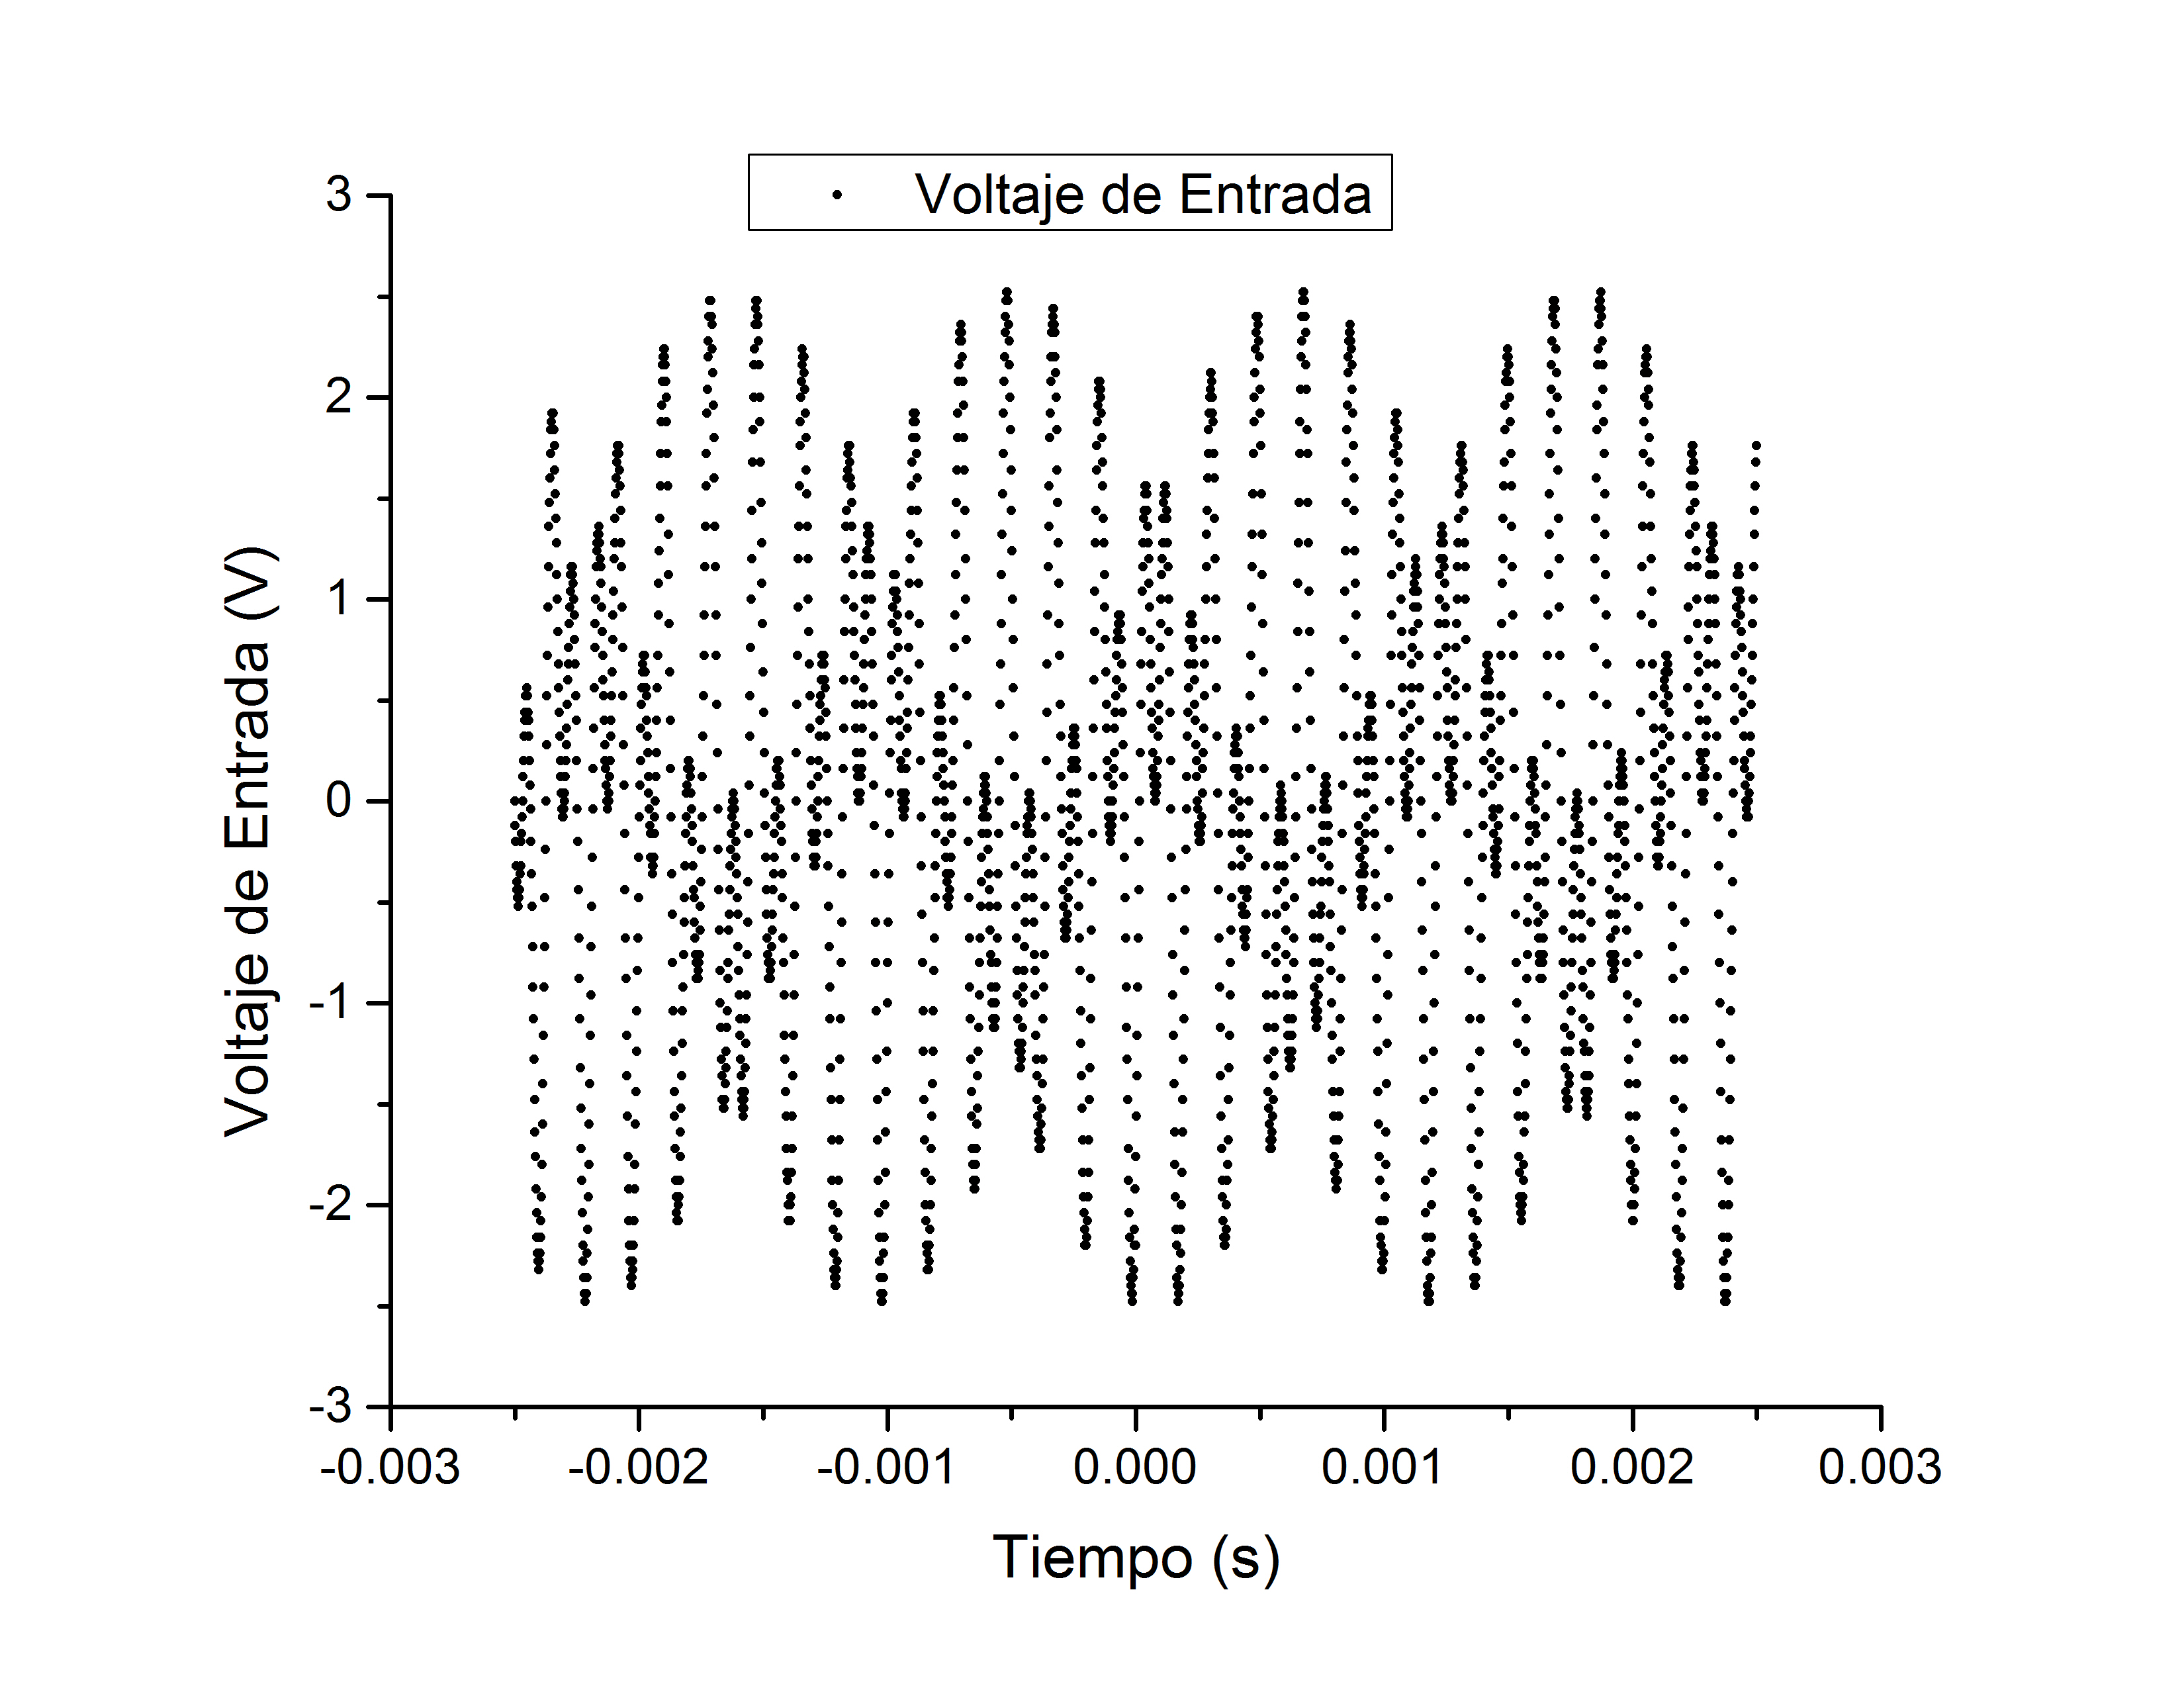
\includegraphics[scale=0.3]{5Khz}
		\subcaption{Señal de entrada del filtro.}
		\label{subfig:5k_NFilt}
	\end{subfigure}
	\begin{subfigure}{0.5\textwidth}
		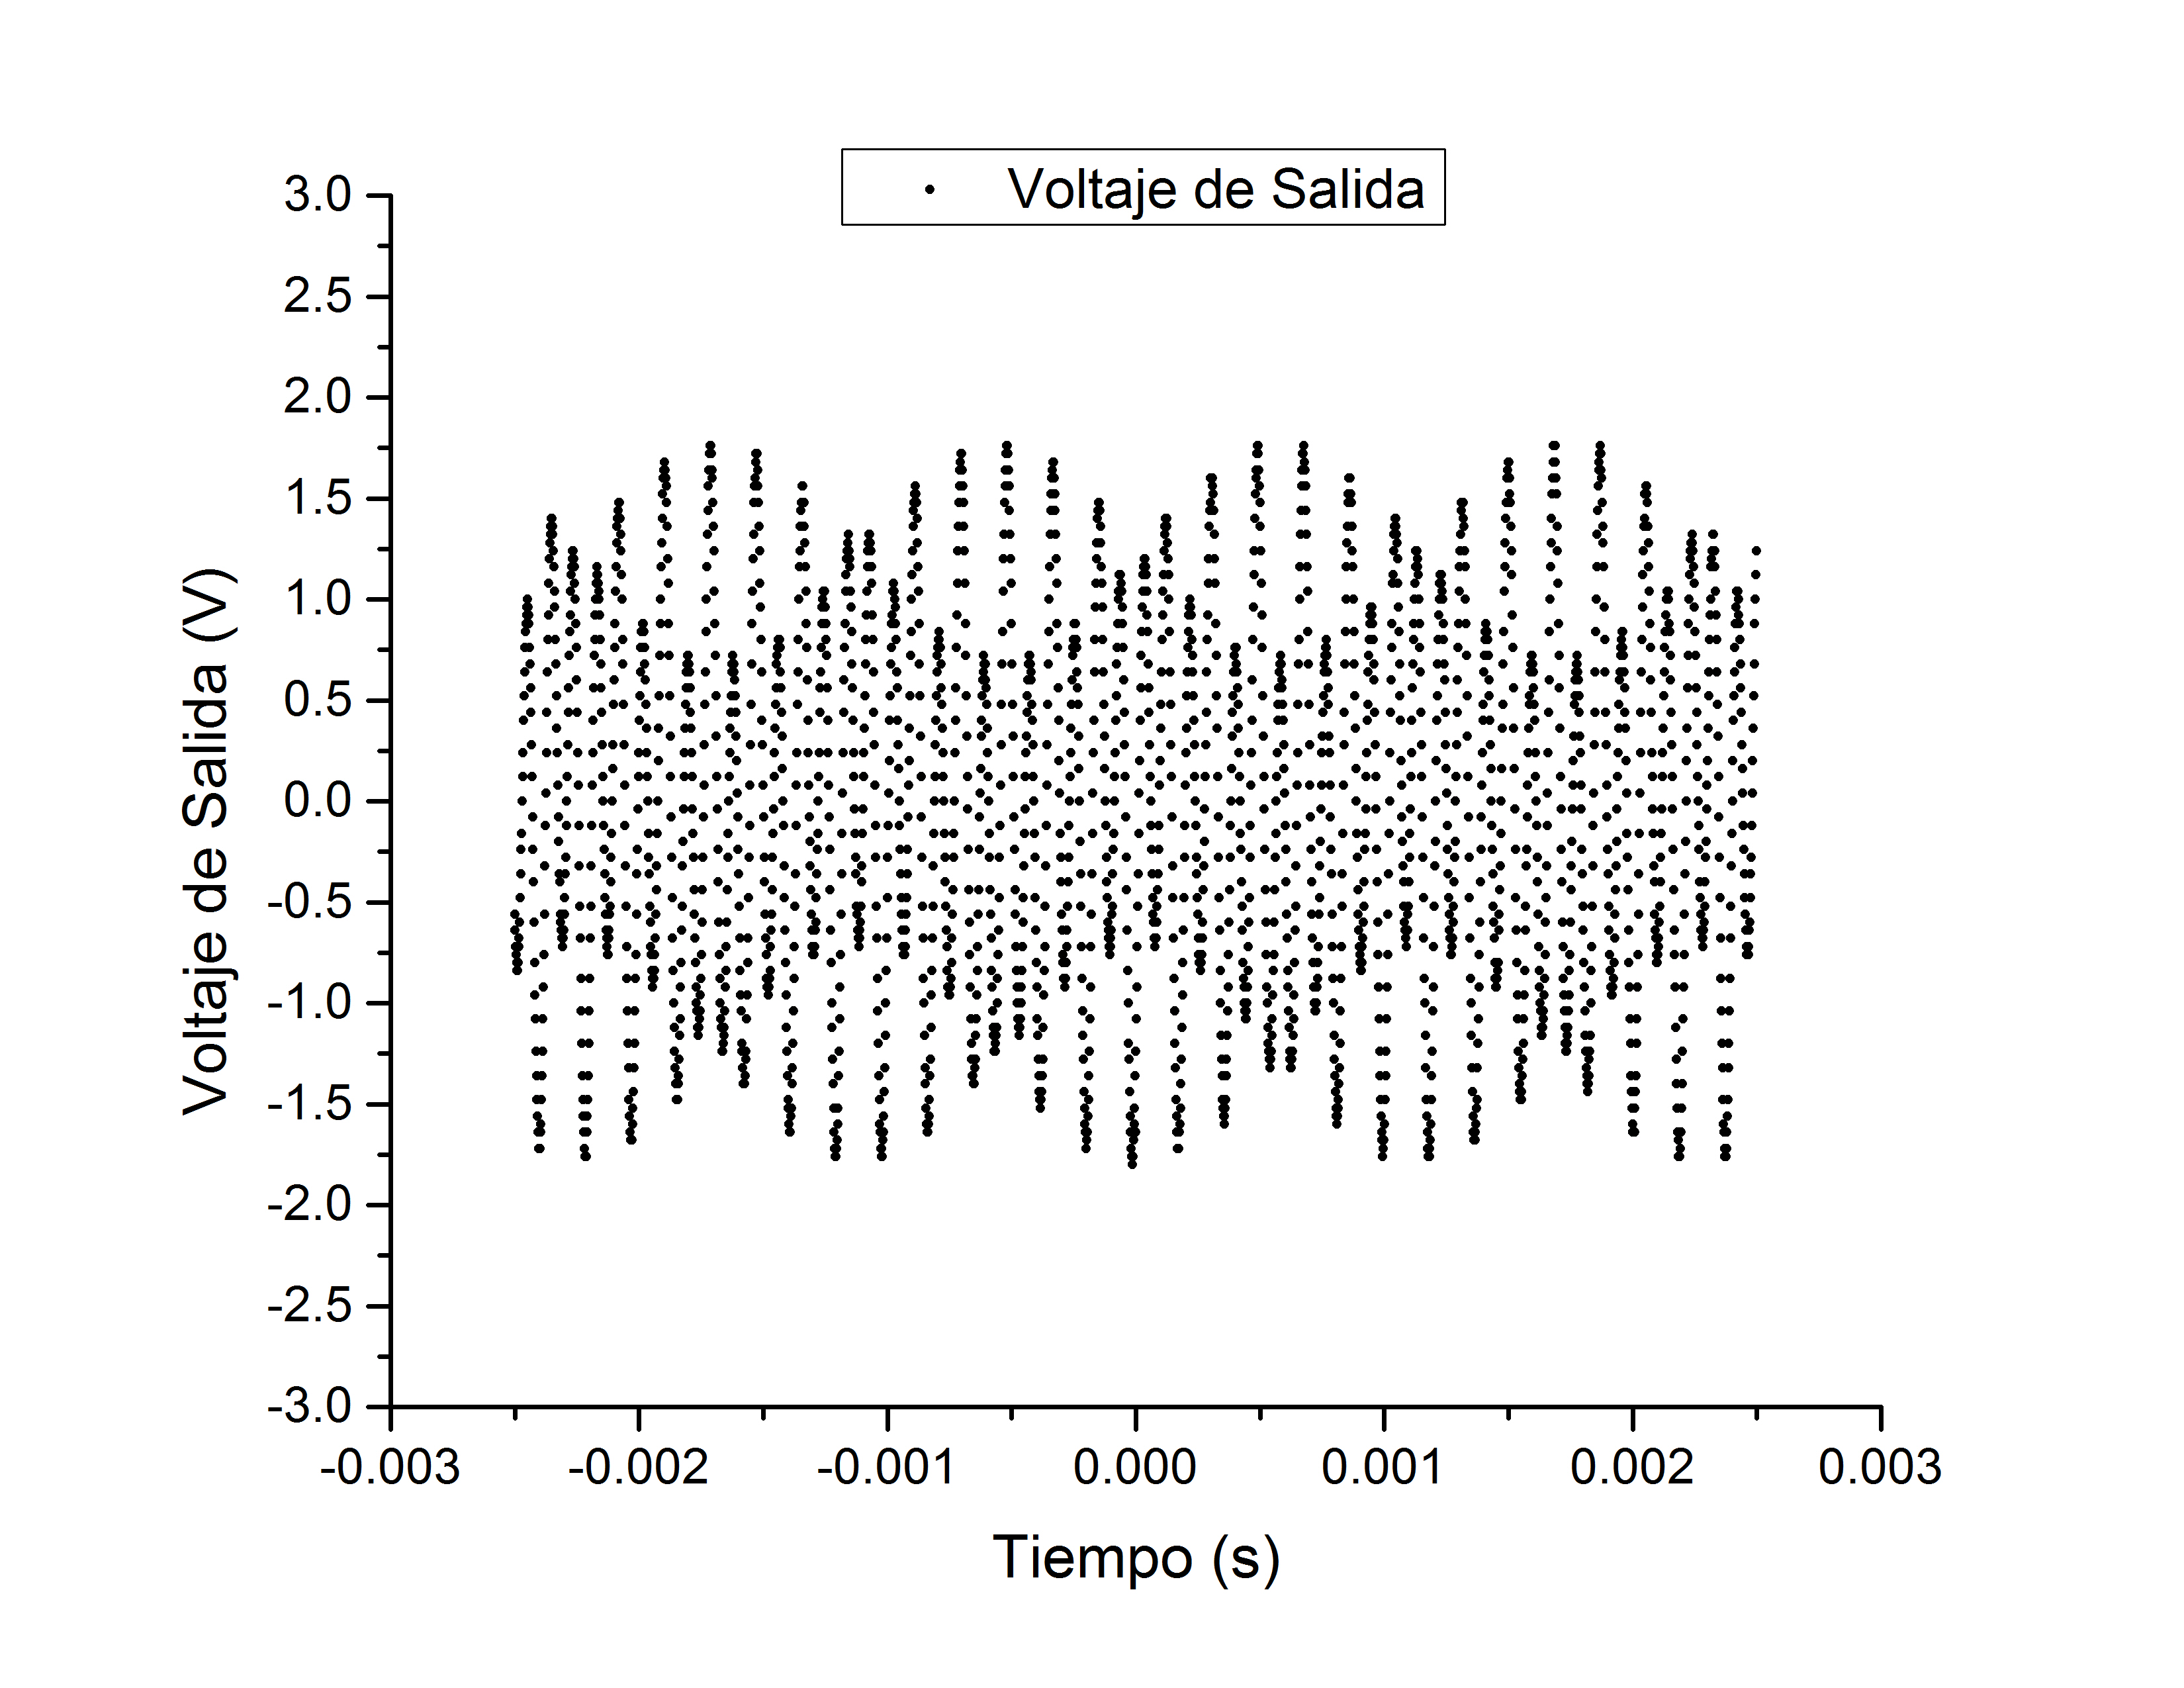
\includegraphics[scale=0.3]{5Khz_Filtrado}
		\subcaption{Señal de salida del filtro.}
		\label{subfig:5k_Filt}
	\end{subfigure}
	\caption{Gráficos que muestran la suma de dos señales sinusoidales, de las cuales una es cercana a la frecuencia de corte del circuito anti-resonante utilizado 
como filtro.}
	\label{fig:5k}
\end{figure}

A diferencia del par anterior, existe una diferencia apreciable entre los gráficos, que es consistente con el hecho de que una de las señales deberia haberse visto afectada por el filtro. Para poder observar mejor eso, se realizo un FFT mediante el programa de procesamiento de datos, OriginLab. La \textbf{Figura \ref{fig:FFT}} muestra los resultados de realizar la \textit{trasformada de Fourier} a cada uno de los graficos anteriores.

\begin{figure}[H]
	\begin{subfigure}{0.5\textwidth}
		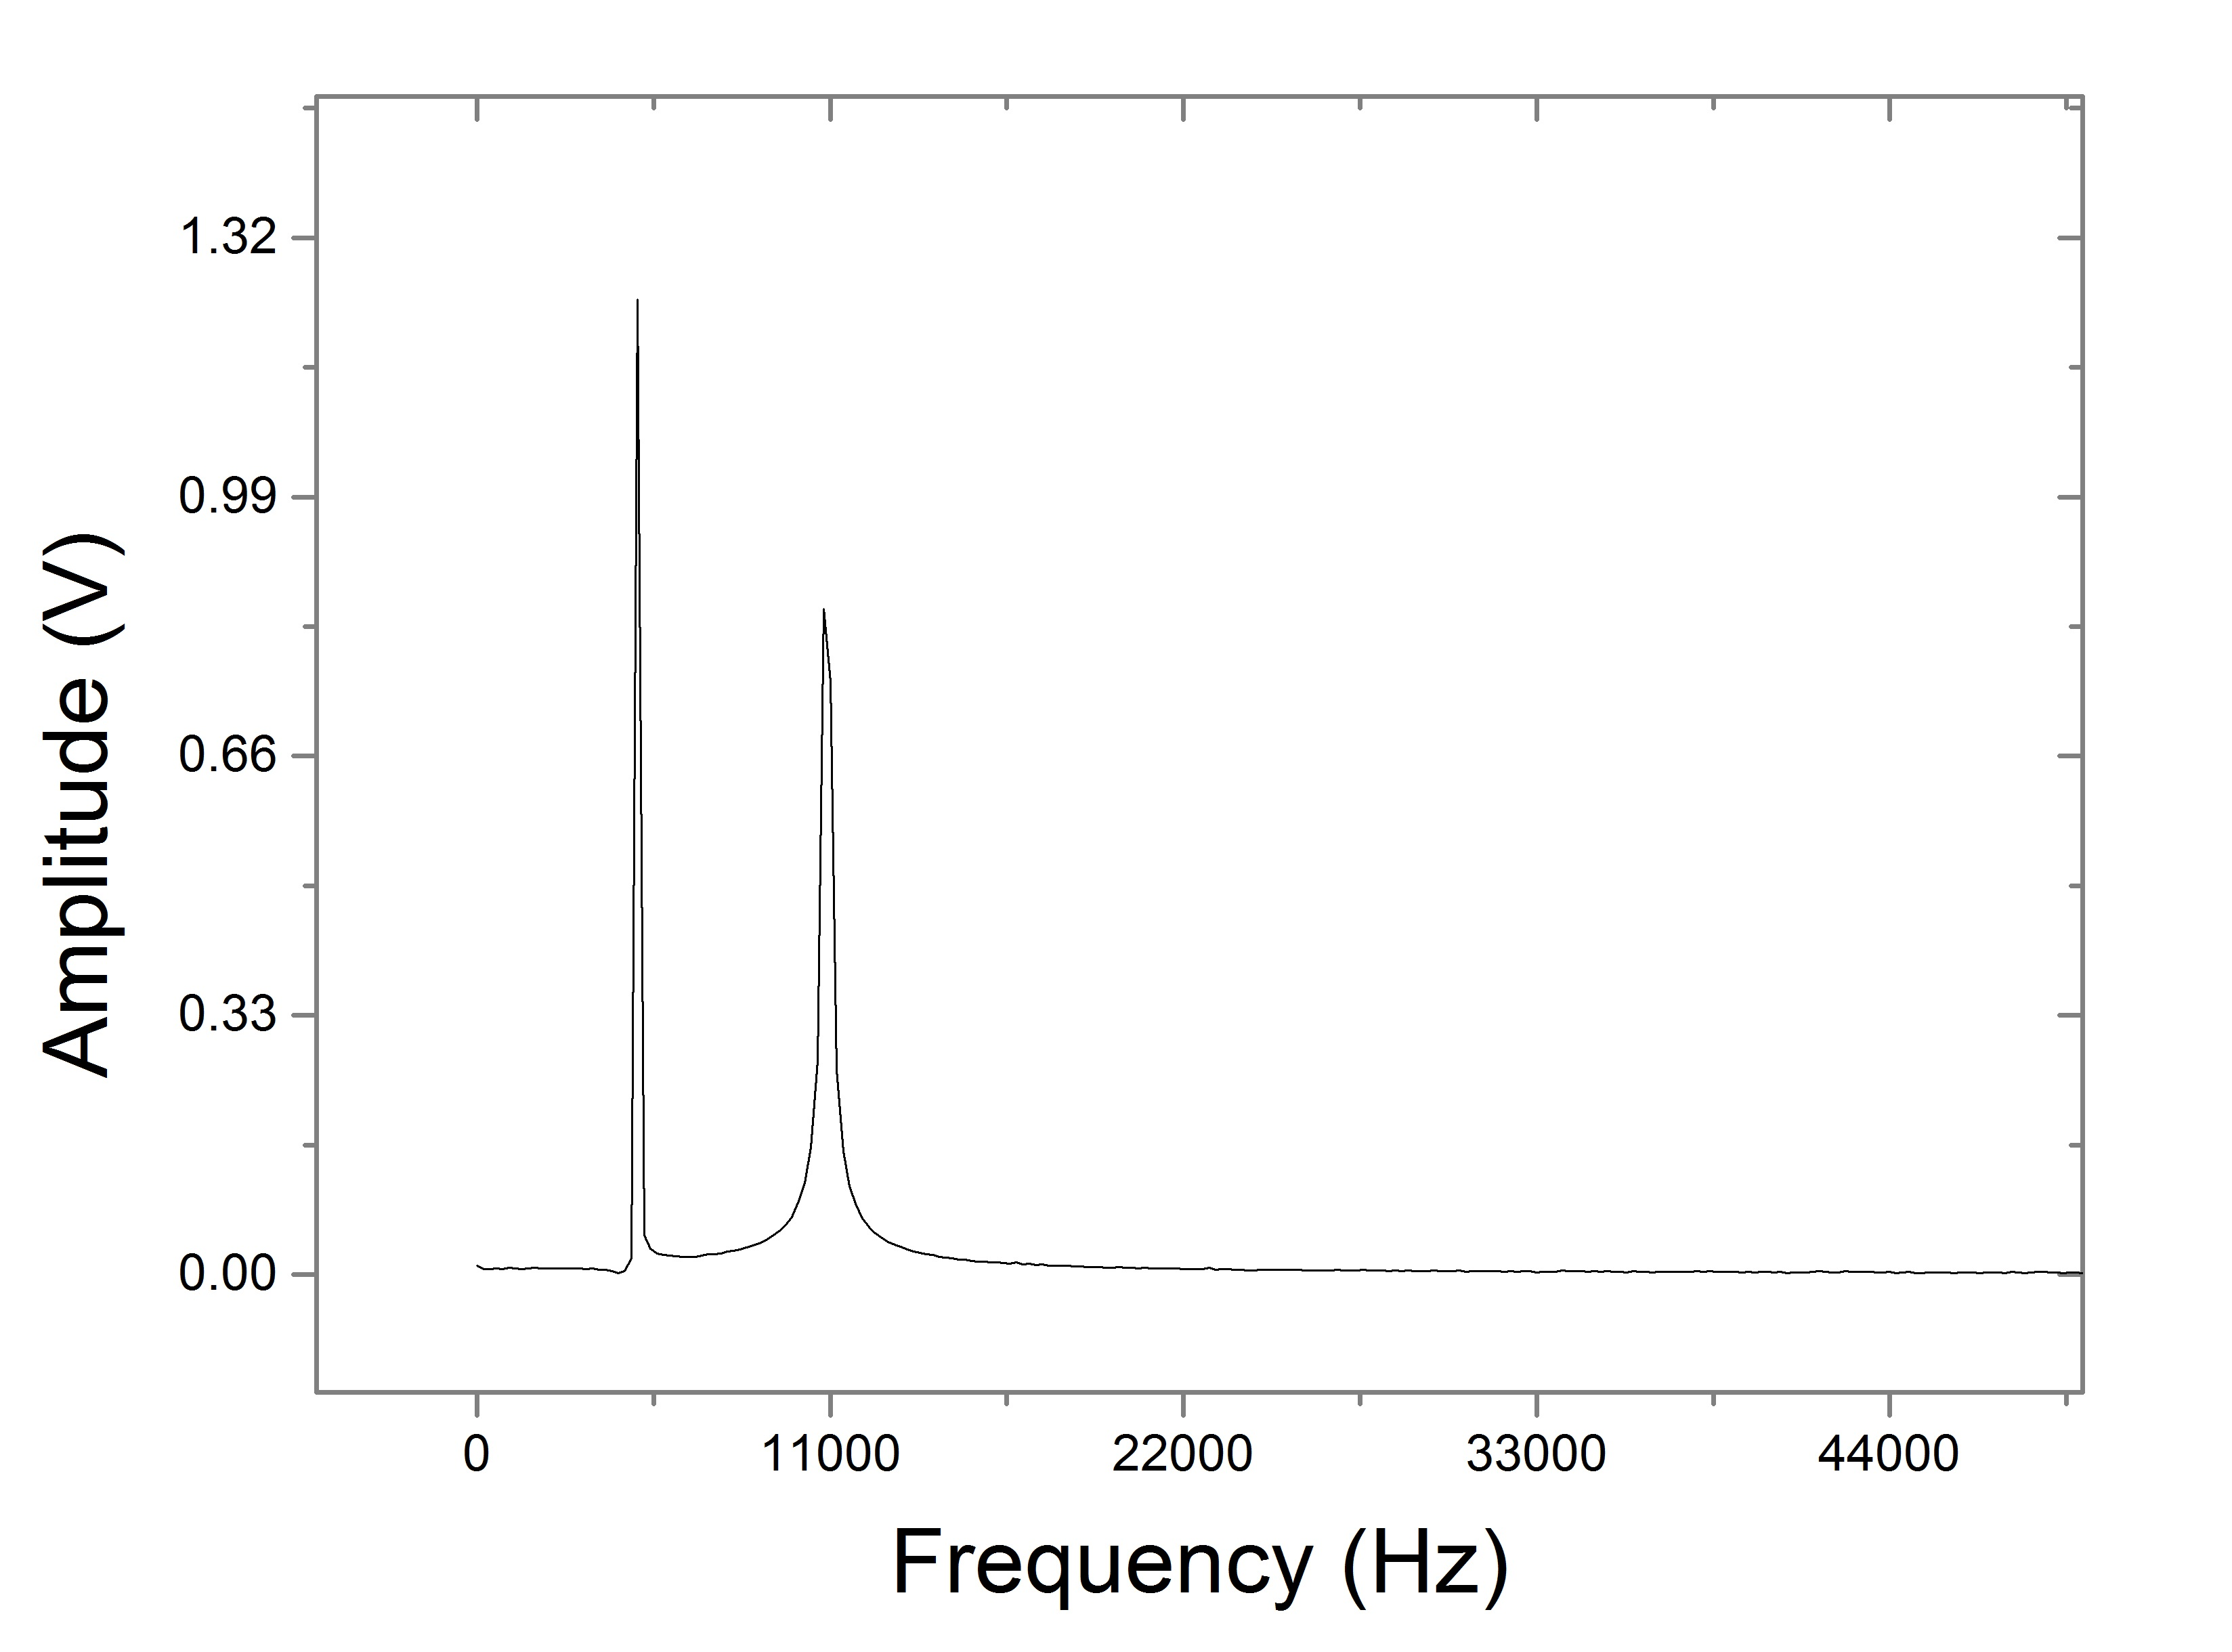
\includegraphics[scale=0.3]{FFT_5005hz}
		\subcaption{Gráfico que corresponde a la transformada de Fourier del grafico de la \textbf{figura \ref{subfig:5k_NFilt}}.}
		\label{subfig:FFT_NFilt}
	\end{subfigure}
	\begin{subfigure}{0.5\textwidth}
		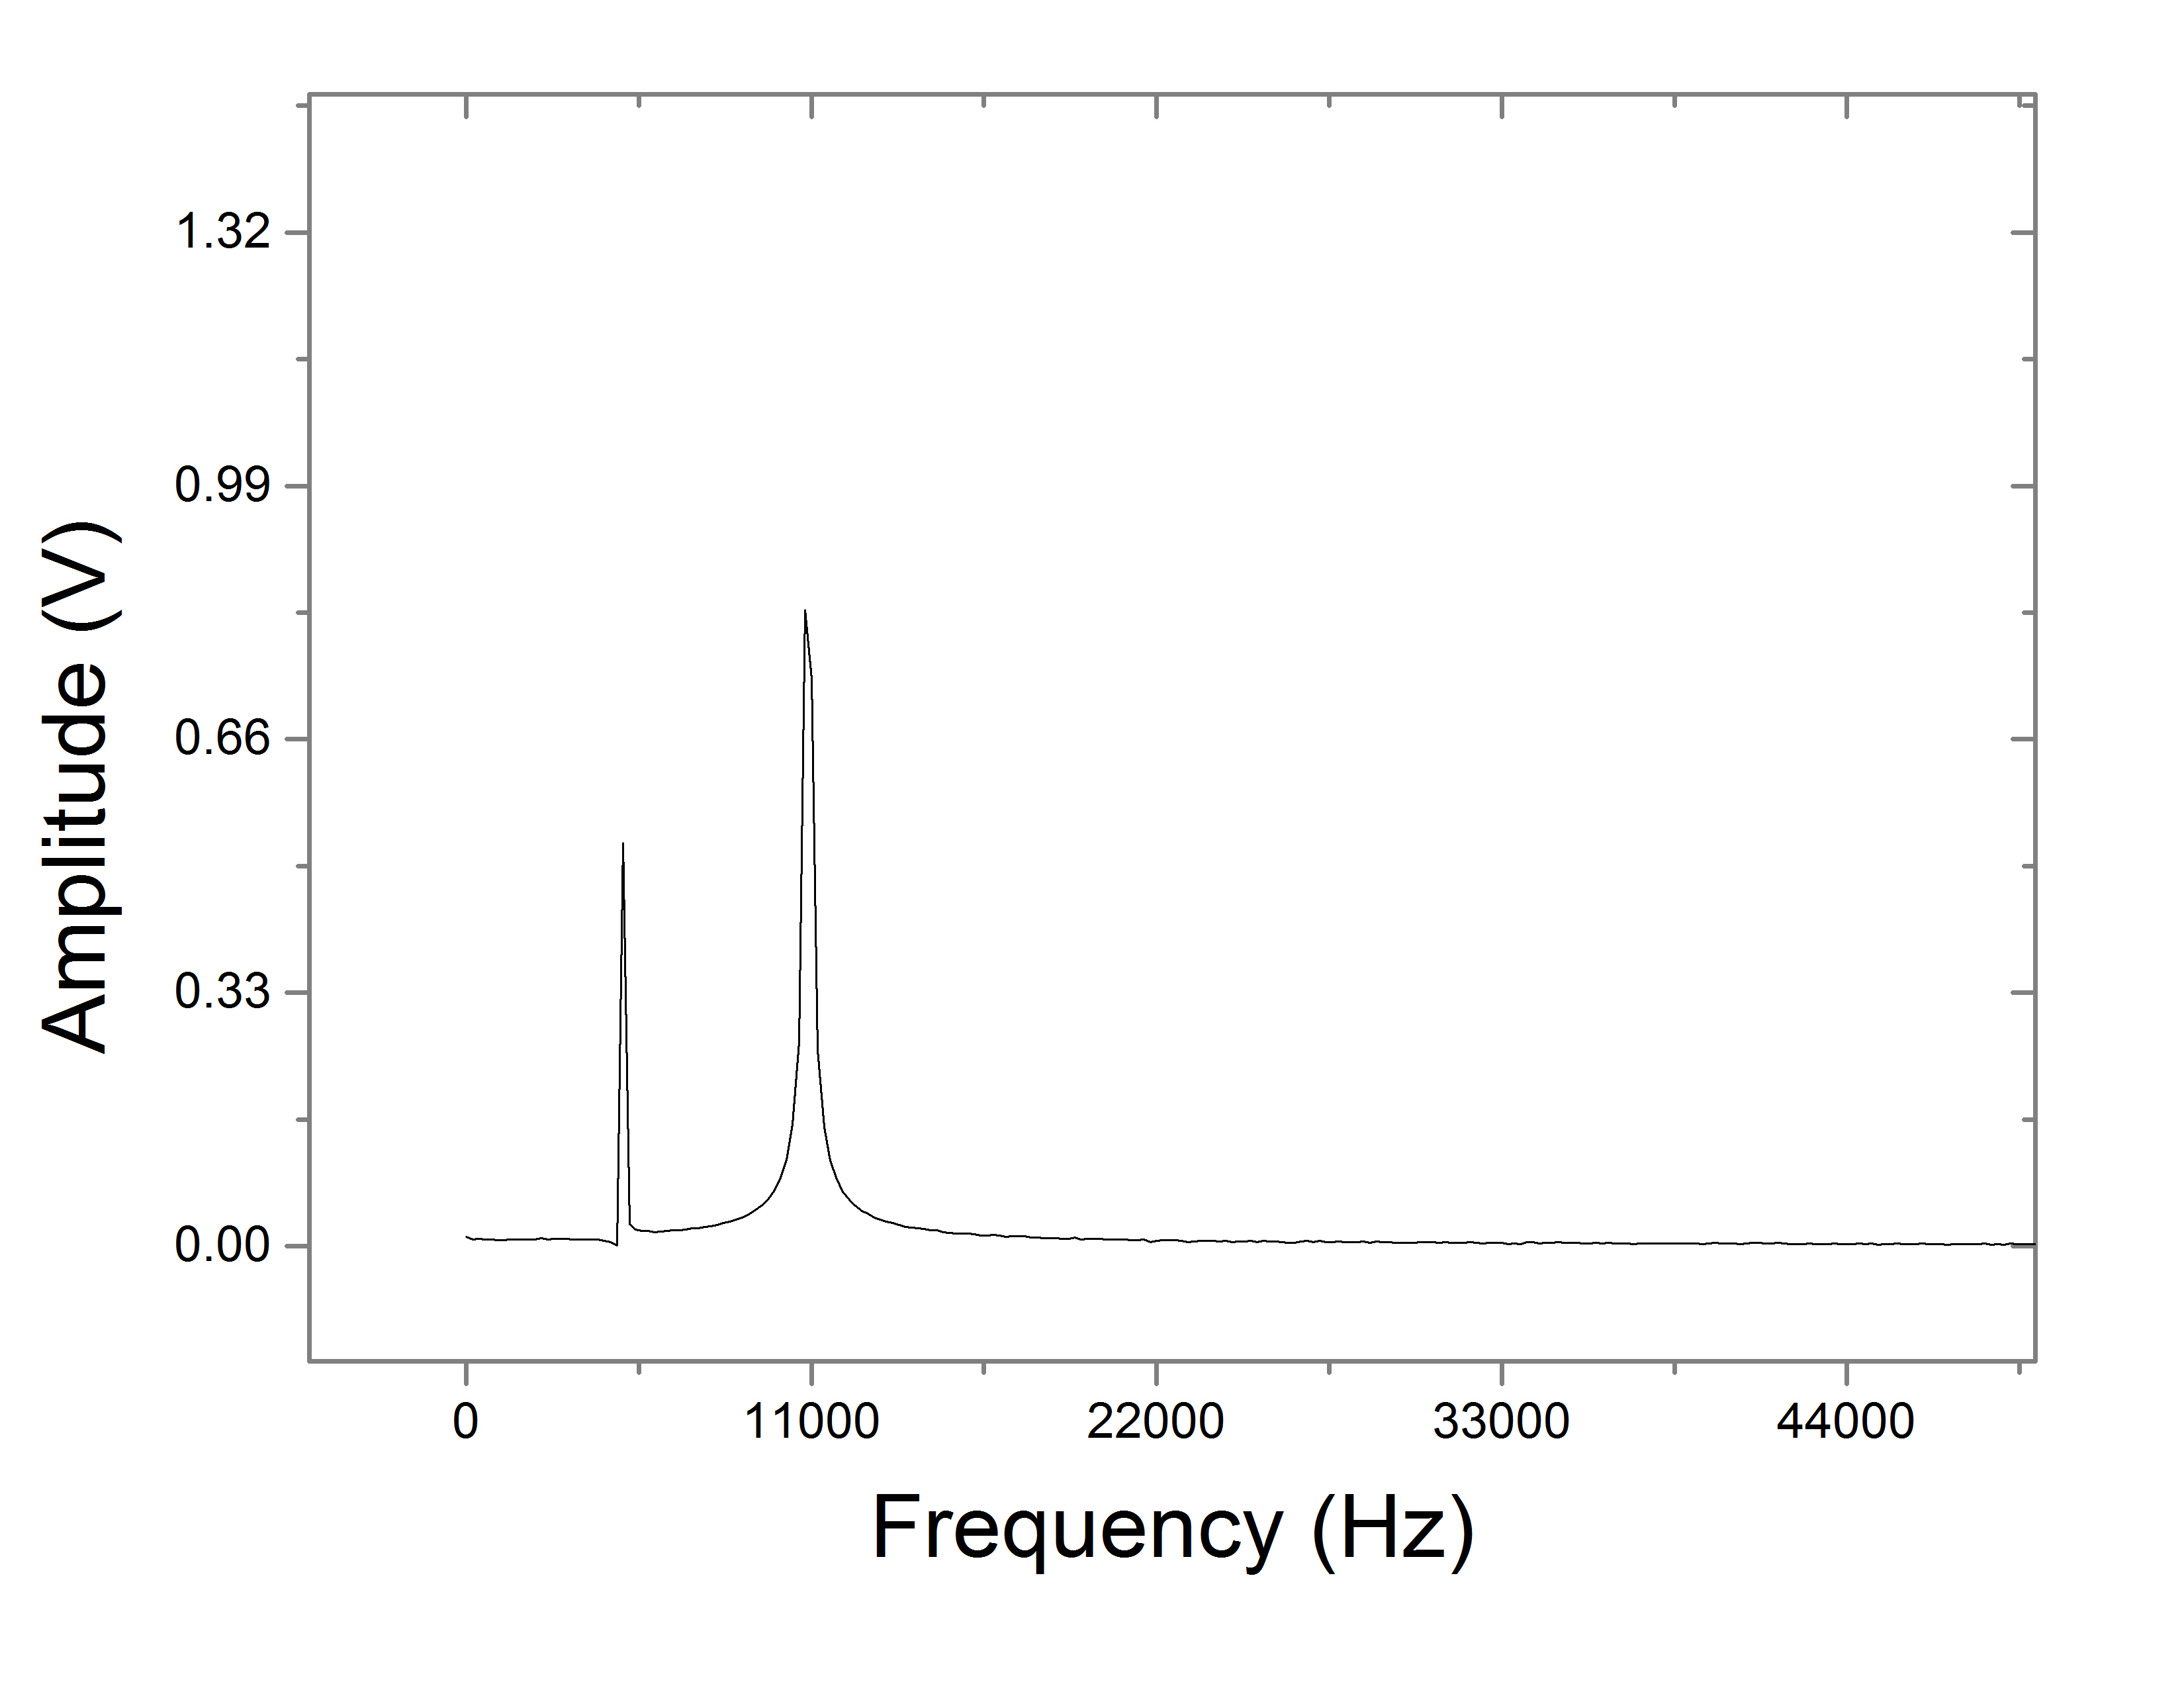
\includegraphics[scale=0.3]{FFT_5005hz_Filtrado}
		\subcaption{Gráfico que correspondiente a la transformada de Fourier del grafico de la \textbf{figura \ref{subfig:5k_NFilt}}.}
		\label{subfig:FFT_Filt}
	\end{subfigure}
	\caption{no se me ocurre un epigrafe para esto.}
	\label{fig:FFT}
\end{figure}

En el gráfico de la \textbf{Figura \ref{subfig:FFT_Filt}} se puede ver como cayo la amplitud de la corriente de frecuencia $f_{baja}= (5005.5 \pm 0.1)hz$ respecto del gráfico de la \textbf{Figura \ref{subfig:FFT_NFilt}}, mientras que la correspondiente a la de frecuencia alta, $f_{alta} = (10844 \pm 1)hz$, se mantiene sin cambios apreciables.

Finalmente se procedio a utilizar el FFT realizado por el osciloscopio para cada medición, y a partir de esos datos se construyó un gráfico que compara la transferencia de las dos señales utilizadas en el \textit{sumador}, variando solo la de frecuencia baja. Los resultados se muestran en la \textbf{figura \ref{fig:Comp}}

\begin{figure}[H]
\centering
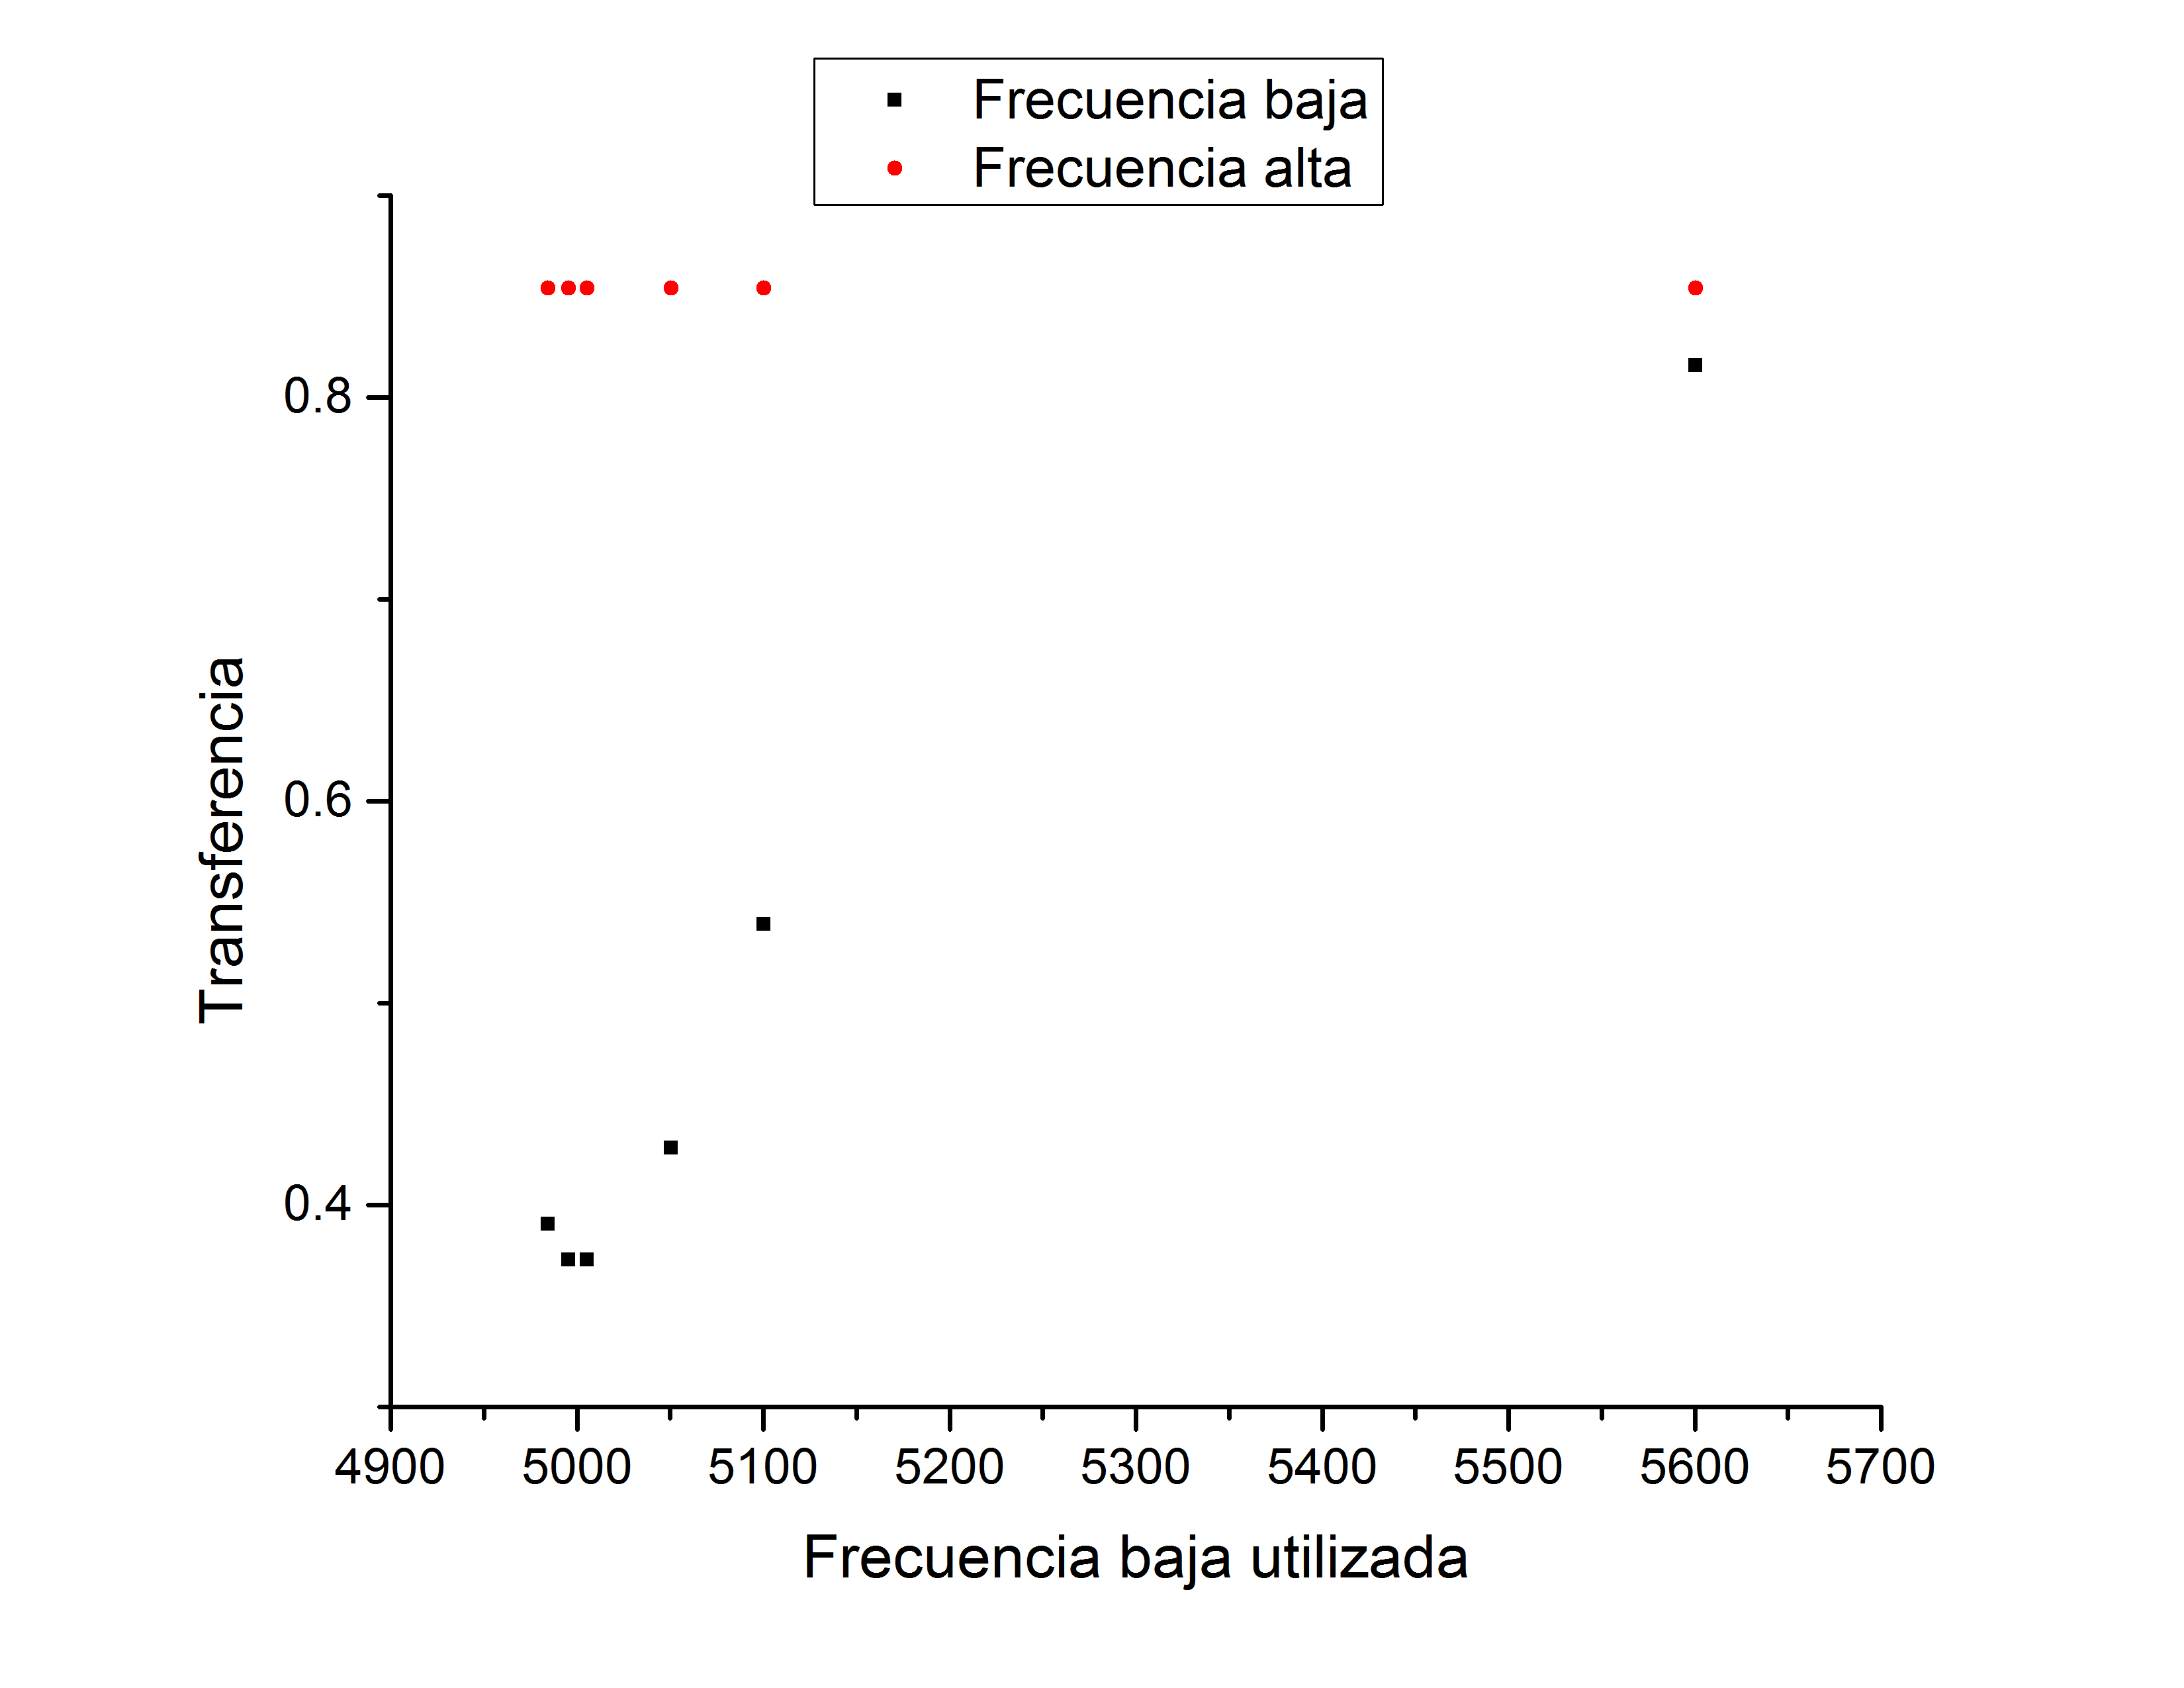
\includegraphics[scale=0.5]{Comparacion}
\caption{Gráfico que compara la transferencia de un circuito RCL anti-resonante para una señal fija, alejada de su campana de anti-resonancia, y para una señal que 
variaba. }
\label{fig:Comp}
\end{figure}

Puede verse en el gráfico \ref{fig:Comp} que la amplitud de la corriente de frecuencia baja aumenta a medida que esta se aleja de la frecuencia de corte, mientras que la señal con frecuencia alta se mantiene sin cambios apreciables.


%%%%%%%%%%%%%%%%%%%%%%%%%%%%%%%%%%%%%%%%%%%%%%%%%%%%%%%%%%%%%%%%%%%%%%%%%%%%%%%%%%%%%%%%%%%%%%%%%%%%%%%%%%%%%%%%%%%%%%%%%%%%%%%%
%	CONCLUSIONES
%%%%%%%%%%%%%%%%%%%%%%%%%%%%%%%%%%%%%%%%%%%%%%%%%%%%%%%%%%%%%%%%%%%%%%%%%%%%%%%%%%%%%%%%%%%%%%%%%%%%%%%%%%%%%%%%%%%%%%%%%%%%%%%%

\section{Conclusiones}
\label{sec:conclusiones}




%%%%%%%%%%%%%%%%%%%%%%%%%%%%%%%%%%%%%%%%%%%%%%%%%%%%%%%%%%%%%%%%%%%%%%%%%%%%%%%%%%%%%%%%%%%%%%%%%%%%%%%%%%%%%%%%%%%%%%%%%%%%%%%%%
%	APÉNDICE: esas cosas extras que simplemente no tuvieron lo suficiente como para ganarse una sección propia.
%%%%%%%%%%%%%%%%%%%%%%%%%%%%%%%%%%%%%%%%%%%%%%%%%%%%%%%%%%%%%%%%%%%%%%%%%%%%%%%%%%%%%%%%%%%%%%%%%%%%%%%%%%%%%%%%%%%%%%%%%%%%%%%%%



%%%%%%%%%%%%%%%%%%%%%%%%%%%%%%%%%%%%%%%%%%%%%%%%%%%%%%%%%%%%%%%%%%%%%%%%%%%%%%%%%%%%%%%%%%%%%%%%%%%%%%%%%%%%%%%%%%%%%%%%%%%%%%%%%
%	REFERENCIAS: libros, libros, libros.
%%%%%%%%%%%%%%%%%%%%%%%%%%%%%%%%%%%%%%%%%%%%%%%%%%%%%%%%%%%%%%%%%%%%%%%%%%%%%%%%%%%%%%%%%%%%%%%%%%%%%%%%%%%%%%%%%%%%%%%%%%%%%%%%%

%Ejemplo:
\begin{thebibliography}{1}
 \bibitem{Berkeley} Frank S. Crawford, \textit{Berkeley physics course 3: Ondas}, 1994, Editorial Reverte S.A.
\end{thebibliography}
%Para citar: blablabla \cite{Baird}
 
\end{document}





